%%%%---------------------------------------------------------------------------------------------------------------
%   PACKAGES
%%%%---------------------------------------------------------------------------------------------------------------

\documentclass[letterpaper,14pt]{book} %two page printing mode
\usepackage{amssymb}
\usepackage{amsmath}
\usepackage{amsfonts}
\usepackage{empheq} %equations environment using amsmath
\usepackage{graphicx}
\usepackage{enumerate}
\usepackage{geometry}
\usepackage{multicol}
\usepackage[ansinew]{inputenc} %auto add accents: ansinew for windwos, latin1 for linux, applemac for macos
\usepackage[spanish]{babel} %spanish words and dashes
\usepackage{verbatim} %use \begin{comment}
\usepackage{amsthm}
\usepackage{mathrsfs}
\usepackage{epsfig}
\usepackage{fancyhdr}
\usepackage{fancybox}
\usepackage{enumitem} %Extended options for List, Numeration and Itemize environments
\usepackage{polynom}
\usepackage{pstricks} %pstricks stuff
\usepackage{pstricks-add} %pstricks stuff
\usepackage{pstricks,pst-node, pst-grad} %pstricks stuff
\usepackage{pstcol} %pstricks stuff
\usepackage{color} %pstricks stuff
\usepackage[labelfont=bf,labelsep=space]{caption} %advanced caption options
\usepackage{float} %activates floating figures
\usepackage[noprefix,refpage,spanish]{nomencl} %symbol list
\usepackage{tocloft} %edit tables names and appearance
\usepackage{centernot} %use to negate log symbols like arcR
\usepackage[none]{hyphenat} %remove hyphenation, use \sloppy to fix overfull lines
\usepackage{bbm} %better R, C, N symbols
\usepackage{textcomp}
\usepackage{nomencl}
\usepackage{mathrsfs}
%%%%---------------------------------------------------------------------------------------------------------------
%   HEADERS AND FOOTERS
%%%%---------------------------------------------------------------------------------------------------------------

\pagestyle{fancy}
\setlength{\headheight}{16pt}
\renewcommand{\chaptermark}[1]{\markboth{\MakeUppercase{#1}}{}}
\fancyhead{} %clear all header fields
\fancyhead[LO]{\textit{N\'UCLEOS POR TRAYECTORIAS MONOCROM\'ATICAS EN DIGR\'AFICAS}}
\fancyhead[RE]{\textit{\leftmark}}
\fancyfoot{} %clear all footer fields
\fancyfoot[CE,CO]{\thepage}
\renewcommand{\headrulewidth}{0.4pt}

%%%%---------------------------------------------------------------------------------------------------------------
%   NAME SWITCHING AND FORMAT
%%%%---------------------------------------------------------------------------------------------------------------

\addto\captionsspanish{\renewcommand{\contentsname}{�ndice}} %\renewcommand{\contentsname}{�ndice} doesn't work, dunno why
\renewcommand{\figurename}{Fig.}
\renewcommand{\proofname}{Demostraci�n}
\renewcommand{\nomname}{�ndice de s�mbolos} %nomenclature shit
\decimalpoint %spanish language interfers with decimal point
\renewcommand{\cftchapdotsep}{4.5} %add dots to index
\renewcommand{\cftfigdotsep}{2} %add dots to figure index
\cftsetindents{figure}{0in}{0.5in} %figure index left side indents

%%%%---------------------------------------------------------------------------------------------------------------
%   THEOREMS
%%%%---------------------------------------------------------------------------------------------------------------

\theoremstyle{plain}
\newtheorem{prox}{Proposici�n}[chapter]
\newtheorem{lemx}[prox]{Lema}
\newtheorem{obsx}[prox]{Observaci�n}
\newtheorem{teox}[prox]{Teorema}
\newtheorem*{teoy}{Teorema} %theorem without number
\newtheorem{defx}{Definici�n}[chapter]
\newtheorem{corox}[prox]{Corolario}
%%%%---------------------------------------------------------------------------------------------------------------
%   MATH SHORTCUTS
%%%%---------------------------------------------------------------------------------------------------------------
\DeclareMathOperator{\arcR}{\longleadsto} %arco
\DeclareMathOperator{\arcL}{\longleftarrow} %arco
\DeclareMathOperator{\arcD}{\longleftleadsto} %arco doble
\DeclareMathOperator{\THEN}{\Rightarrow} %implica
\DeclareMathOperator{\RR}{\mathbbm{R}} %numeros reales
\DeclareMathOperator{\NN}{\mathbbm{N}} %numeros naturales
%\DeclareMathOperator{\CCC}{\mathcal{C}} %
%\DeclareMathOperator{\CCCC}{\mathfrak{C}} %

%%%%---------------------------------------------------------------------------------------------------------------
%   SYMBOL LIST BULLSHIT 
%%%%---------------------------------------------------------------------------------------------------------------

%-------------------------------------------------------
% INSERTAR AQUI TITULO DEL ARCHIVO DE TESIS
%-------------------------------------------------------

\makeindex
\def\execute{%
\begingroup
\catcode`\%=12
\catcode`\\=12
\executeaux}
\def\executeaux#1{\immediate\write18{#1}\endgroup}
\execute{makeindex XENTRIX.nlo -s nomencl.ist -o XENTRIX.nls}
\makenomenclature
\setlength{\nomitemsep}{0.05cm}
\renewcommand{\pagedeclaration}[1]{\dotfill\nobreakspace#1}

%%%%---------------------------------------------------------------------------------------------------------------
%   BRIEF TITLE
%%%%---------------------------------------------------------------------------------------------------------------

\title{N\'ucleos por trayectorias monocrom\'aticas en digr\'aficas}
\author{Jos\'e Mu\~noz Porras}
\date{2011}

%%%%---------------------------------------------------------------------------------------------------------------
%   BEGIN!
%%%%---------------------------------------------------------------------------------------------------------------
\setlength{\headheight}{30.3pt}

\begin{document}
\newrgbcolor{ttqqcc}{0.2 0 0.8}
\newrgbcolor{ffwwqq}{1 0.4 0}
\newrgbcolor{qqttqq}{0 0.2 0}
\newrgbcolor{qqqqzz}{0 0 0.6}
\newrgbcolor{ttttqq}{0.2 0.2 0}
\newrgbcolor{qqqqcc}{0 0 0.8}
\newrgbcolor{zzttqq}{0.6 0.2 0}
\newrgbcolor{xdxdff}{0.49 0.49 1}
\newrgbcolor{ttwwqq}{0.2 0.4 0}
\newrgbcolor{ccqqqq}{0.8 0 0}
\newrgbcolor{ccccqq}{0.8 0.8 0}
\newrgbcolor{ccqqcc}{0.8 0 0.8}
%%%%---------------------------------------------------------------------------------------------------------------
%   COVER + BLANK PAGE
%%%%---------------------------------------------------------------------------------------------------------------


%%%%---------------------------------------------------------------------------------------------------------------
%   TITLE PAGE + BLANK PAGE
%%%%---------------------------------------------------------------------------------------------------------------


%%%%---------------------------------------------------------------------------------------------------------------
%   DATA SHEET (What a shitty piece of code) + BLANK PAGE
%%%%---------------------------------------------------------------------------------------------------------------



%%%%---------------------------------------------------------------------------------------------------------------
%   QUOTE + BLANK PAGE
%%%%---------------------------------------------------------------------------------------------------------------
%%%%---------------------------------------------------------------------------------------------------------------
%   PRELUDE
%%%%---------------------------------------------------------------------------------------------------------------

\frontmatter
\sloppy

%%%%---------------------------------------------------------------------------------------------------------------
%   THANKS
%%%%---------------------------------------------------------------------------------------------------------------

%%%%---------------------------------------------------------------------------------------------------------------
%   TABLE OF CONTENTS
%%%%---------------------------------------------------------------------------------------------------------------


%%%%---------------------------------------------------------------------------------------------------------------
%   INTRODUCTION
%%%%---------------------------------------------------------------------------------------------------------------

\chapter{Introducci�n}
%%%%---------------------------------------------------------------------------------------------------------------
%   THESIS
%%%%---------------------------------------------------------------------------------------------------------------

\mainmatter

%%%%---------------------------------------------------------------------------------------------------------------
%   CHAPTER ONE
%%%%---------------------------------------------------------------------------------------------------------------
\chapter{Definiciones}

Una \emph{gr\'afica dirigida}, o \emph{digr\'afica}, $D$ consiste de un conjunto de v\'ertices no vac\'io y de un conjunto de parejas ordenadas de v\'ertices distintos llamadas flechas. Usaremos la siguiente notaci\'on: \\
Sea $D=(V,A)$ una digr\'afica. $V$ denota el conjunto de v\'ertices y $A$ el de flechas de D. 
\begin{figure}[h!!t]
\begin{center}
\begin{pspicture}(-7.0,-1.86)(8.38,4.3)
\psset{xunit=1.0cm,yunit=1.0cm,algebraic=true,dotstyle=o,dotsize=3pt 0,linewidth=1pt,arrowsize=5pt 2,arrowinset=0.25}
\psline{->}(-1.2,3.4)(0.64,4.72)
\psline{->}(-1.2,3.4)(-0.51,1.24)
\psline{->}(0.64,4.72)(2.46,3.38)
\psline{->}(2.46,3.38)(-1.2,3.4)
\psline{->}(-0.51,1.24)(2.47,3.38)
\psline{->}(0.46,-0.86)(-0.51,1.24)
\psline{->}(2.46,3.38)(1.75,1.23)
\psline{->}(1.75,1.23)(-0.51,1.24)
\parametricplot{1.358652573790421}{3.2160814438036747}{1*1.33*cos(t)+0*1.33*sin(t)+0.16|0*1.33*cos(t)+1*1.33*sin(t)+3.5}
\psdots[dotsize=8pt 0,dotstyle=triangle*,linecolor=blue](0.44,4.8)
\psdots[dotstyle=*,linecolor=blue](0.64,4.72)
\psdots[dotstyle=*,linecolor=blue](-1.2,3.4)
\psdots[dotstyle=*,linecolor=darkgray](-0.51,1.24)
\psdots[dotstyle=*,linecolor=darkgray](1.75,1.23)
\psdots[dotstyle=*,linecolor=darkgray](2.46,3.38)
\psdots[dotstyle=*,linecolor=blue](0.46,-0.86)
\rput[bl](0.72,4.84){\blue{$u$}}
\rput[bl](2.72,3.38){\blue{$v$}}
\rput[bl](-1.62,3.36){\blue{$x_1$}}
\rput[bl](-0.96,1.16){\blue{$x_2$}}
\rput[bl](1.88,0.98){\blue{$x_4$}}
\rput[bl](0.38,-1.2){\blue{$x_3$}}
\end{pspicture}
\caption{Una digr\'afica.}
\label{generada}
\end{center}
\end{figure}

El \emph{orden} de $D$ es el n\'umero de v\'ertices en $D$, es decir, la cardinalidad de $D$. Por ejemplo, el orden de la digr\'afica en la figura 1.1 es 6. \\
Para una flecha $(u,v)$, decimos que $u$ es in-vecino de $v$, o que $u$ es ex-vecino de $v$. Si $(u,v)$ es una flecha tambi\'en decimos que $v$ \emph{absorbe} a $u$, y que  $u$ \emph{domina} a $v$. \\
Sea $D$ una digr\'afica. Una flecha $(u,v)\in A(D)$ es \emph{sim\'etrica} si existe $(v,u) \in A(D)$. Si \emph{todas} las flechas de una digr\'afica $D$ son sim\'etricas, decimos que $D$ es \emph{sim\'etrica}. Si \emph{ninguna} flecha de $D$ es sim\'etrica entonces decimos que $D$ es \emph{asim\'etrica}.  \\
Vamos a utilizar la notaci\'on $[u,v] \in A(D)$ para denotar que $(u,v) \in A(D)$ o que $(v,u) \in A(D)$. \\ 
\begin{figure}[h!!t]
\begin{center}
\begin{pspicture}(-7.0,0)(8.38,5)
\psset{xunit=1.0cm,yunit=1.0cm,algebraic=true,dotstyle=o,dotsize=3pt 0,linewidth=1pt,arrowsize=5pt 2,arrowinset=0.25}
\psline{->}(0.66,4.72)(-1.18,3.4)
\parametricplot{1.358652573790421}{3.2160814438036747}{1*1.33*cos(t)+0*1.33*sin(t)+0.16|0*1.33*cos(t)+1*1.33*sin(t)+3.5}
\psline{->}(1.77,1.23)(2.48,3.38)
\psline{->}(-1.18,3.4)(-0.49,1.24)
\parametricplot{-1.1818394466158892}{0.717083765430057}{1*1.32*cos(t)+0*1.32*sin(t)+1.5|0*1.32*cos(t)+1*1.32*sin(t)+2.52}
\parametricplot{2.5045223243141095}{4.591193057002121}{1*1.24*cos(t)+0*1.24*sin(t)+-0.34|0*1.24*cos(t)+1*1.24*sin(t)+2.5}
\psdots[dotstyle=*,linecolor=blue](0.66,4.72)
\rput[bl](0.66,4.92){\blue{$v$}}
\psdots[dotstyle=*,linecolor=blue](-1.18,3.4)
\rput[bl](-1.42,3.5){\blue{$u$}}
\psdots[dotstyle=*,linecolor=darkgray](-0.49,1.24)
\psdots[dotstyle=*,linecolor=darkgray](1.77,1.23)
\psdots[dotstyle=*,linecolor=darkgray](2.48,3.38)
\psdots[dotsize=4pt 0,dotstyle=triangle*,linecolor=blue](0.44,4.8)
\psdots[dotsize=4pt 0,dotstyle=triangle*,linecolor=blue](2,1.3)
\psdots[dotsize=4pt 0,dotstyle=triangle*,dotangle=90,linecolor=blue](-1.34,3.24)
\end{pspicture}
\caption{Una digr\'afica sim\'etrica.}
\label{generada}
\end{center}
\end{figure}


Sea $D = (V, A)$ una digr\'afica. Sea $K \subset V$. Decimos que $K$ es un \emph{conjunto independiente} de V, si para cualesquiera $u,v\in K$ no existe ni $(u,v)$  ni $(v,u) \in A$. Si cada v\'ertice que no est\'a en $K$ es absorbido por un v\'ertice en K decimos que K es un \emph{conjunto absorbente} de v\'ertices. Si $K$ es independiente y dominante decimos que $K$ es un \emph{n\'ucleo} de $D$.\\ 

Dada una digr\'afica $D$, una \emph{subdigr\'afica} de $D$ es la digr\'afica que se forma si tomamos un subconjunto de v\'ertices de D y tomamos todas las flechas que tienen como v\'ertices iniciales o terminales uno de esos v\'ertices. \\


Por ejemplo, la digr\'afica de la Figura 1.3 es subdigr\'afica de la de la Figura 1.2\\. 
Una \emph{digr\'afica inducida} por un conjunto de v\'ertices $V' \subseteq V$, denotada por $D[V']$, es la digr\'afica que tiene como conjunto de v\'ertices a $V'$ y que contiene a todos las flechas que contiene $A$ sobre ese conjunto de v\'ertices. \\ 
\begin{figure}[h!!t]
\begin{center}
\begin{pspicture}(-6.5,2.5)(8.38,5.3)
\psset{xunit=1.0cm,yunit=1.0cm,algebraic=true,dotstyle=o,dotsize=3pt 0,linewidth=1pt,arrowsize=5pt 2,arrowinset=0.25}
\psline{->}(0.66,4.72)(-1.18,3.4)
\parametricplot{1.358652573790421}{3.2160814438036747}{1*1.33*cos(t)+0*1.33*sin(t)+0.16|0*1.33*cos(t)+1*1.33*sin(t)+3.5}
\psdots[dotstyle=*,linecolor=blue](0.66,4.72)
\rput[bl](0.66,4.92){\blue{$v$}}
\psdots[dotstyle=*,linecolor=blue](-1.18,3.4)
\rput[bl](-1.54,3.34){\blue{$u$}}
\psdots[dotsize=8pt 0,dotstyle=triangle*,linecolor=blue](0.44,4.8)
\end{pspicture}
\caption{Una subgr\'afica inducida por un conjunto de v\'ertices.}
\label{generada}
\end{center}
\end{figure}

Una gr\'afica es \emph{completa} si para todo par de v\'ertices $u,v$ existe $(u,v)\in A(D)$. \\
La \emph{gr\'afica subyacente} de una digr\'afica $D = (V,A)$, es la gr\'afica que tiene como conjunto de v\'ertices a V, y $u$ y $v$ son adyacentes, si y solo si, $(u,v)\in A(D)$ o $(v,u) \in A(D)$. \\
Una digr\'afica es \emph{semicompleta} si su gr\'afica subyacente es completa.
\begin{figure}[h!!t]
\begin{center}
\begin{pspicture}(-7,0.86)(8.38,4.5)
\psset{xunit=1.0cm,yunit=1.0cm,algebraic=true,dotstyle=o,dotsize=3pt 0,linewidth=1pt,arrowsize=4pt 2,arrowinset=0.25}
\psline{->}(0.66,4.72)(-1.18,3.4)
\psline{->}(0.66,4.72)(2.48,3.38)
\psline{->}(1.77,1.23)(-0.49,1.24)
\psline{->}(1.77,1.23)(2.48,3.38)
\psline{->}(-1.18,3.4)(-0.49,1.24)
\psline{->}(0.66,4.72)(1.77,1.23)
\psline{->}(2.48,3.38)(-1.18,3.4)
\psline{->}(-0.49,1.24)(0.66,4.72)
\psline{->}(-1.18,3.4)(1.77,1.23)
\psline{->}(-0.49,1.24)(2.49,3.38)
\psdots[dotstyle=*,linecolor=blue](0.66,4.72)
\rput[bl](0.66,4.92){\blue{$v$}}
\psdots[dotstyle=*,linecolor=blue](-1.18,3.4)
\rput[bl](-1.42,3.5){\blue{$u$}}
\psdots[dotstyle=*,linecolor=darkgray](-0.49,1.24)
\psdots[dotstyle=*,linecolor=darkgray](1.77,1.23)
\psdots[dotstyle=*,linecolor=darkgray](2.48,3.38)
\end{pspicture}
\caption{Un torneo.}
\label{generada}
\end{center}
\end{figure}

Un \emph{torneo} es una gr\'afica dirigida obtenida al asignar una direcci\'on a cada arista en una gr\'afica completa. \\
Una digr\'afica $D$ es \emph{m-coloreable} si las flechas de $D$ son coloreadas por $m$ colores.  
\begin{figure}[h!!t]
\begin{center}
\begin{pspicture}(-7,-1.86)(8.38,5.3)
\psset{xunit=1.0cm,yunit=1.0cm,algebraic=true,dotstyle=o,dotsize=3pt 0,linewidth=1pt,arrowsize=4pt 2,arrowinset=0.25}
\psline[linecolor=red]{->}(0.66,4.72)(-1.18,3.4)
\psline[linecolor=ttqqcc]{->}(0.66,4.72)(2.48,3.38)
\psline[linecolor=ttqqcc]{->}(0.66,4.72)(2.48,3.38)
\psline[linecolor=green]{->}(1.77,1.23)(-0.49,1.24)
\psline[linecolor=ttqqcc]{->}(1.77,1.23)(2.48,3.38)
\psline[linecolor=red]{->}(-1.18,3.4)(-0.49,1.24)
\psline[linecolor=green]{->}(0.66,4.72)(1.77,1.23)
\psline[linecolor=red]{->}(2.48,3.38)(-1.18,3.4)
\psline[linecolor=red]{->}(-0.49,1.24)(0.66,4.72)
\psline[linecolor=green]{->}(-1.18,3.4)(1.77,1.23)
\psline[linecolor=green]{->}(-0.49,1.24)(2.49,3.38)
\psline[linecolor=ttqqcc]{->}(-0.49,1.24)(-1.6,-0.64)
\psline[linecolor=red]{->}(1.77,1.23)(-1.6,-0.64)
\psline[linecolor=ttqqcc]{->}(2.48,3.38)(4.52,3.34)
\psdots[dotstyle=*,linecolor=blue](0.66,4.72)
\rput[bl](0.66,4.92){\blue{$v$}}
\psdots[dotstyle=*,linecolor=blue](-1.18,3.4)
\rput[bl](-1.42,3.5){\blue{$u$}}
\psdots[dotstyle=*,linecolor=darkgray](-0.49,1.24)
\psdots[dotstyle=*,linecolor=darkgray](1.77,1.23)
\psdots[dotstyle=*,linecolor=darkgray](2.48,3.38)
\psdots[dotstyle=*,linecolor=blue](-1.6,-0.64)
\rput[bl](-1.52,-0.52){\blue{$A$}}
\psdots[dotstyle=*,linecolor=blue](4.52,3.34)
\end{pspicture}
\caption{Una digr\'afica 3-coloreable.}
\label{generada}
\end{center}
\end{figure}
Una \emph{trayectoria dirigida} en $D$ es una secuencia alternante $W=x_1 a_1 x_2 a_2 \ldots x_{k-1}a_{k-1}x_k$ de v\'ertices $x_i$ y flechas $a_j$ en $D$ tales que para todo $i$, $a_i$ sale de $x_i$ y llega a $x_{i+1}$. \\ 
A una trayectoria de $u$ a $v$ le podemos asignar el nombre de \emph{$uv$-trayectoria}. Una $uv-$trayectoria la vamos a denotar tambi\'en por $u \leadsto v$ \\
Si en una $uv$-trayectoria todas las flechas tienen el mismo color decimos que es una trayectoria monocrom\'atica. Vamos a representar una $uv-$trayectoria monocrom\'atica como $u \leadsto_m v$ \\
Sea $D$ una digr\'afica. Decimos que $C_k$ es un \emph{c\'iclo} en $D$ si $C_k$ es una trayectoria que inicia y termina en el mismo v\'ertice. $C_k=(u_0,u_1,\ldots,u_{k-1})$. \\
Vamos a denotar al c\'iclo de tres v\'ertices por $C_3$ y al torneo transtivo de tres v\'ertices por $TT_3$. Los vamos a llamar indistintamente \emph{tri\'angulos}.\\
\begin{figure}[h!!t]
\begin{center}
\begin{pspicture}(-3.19,-1.05)(6.3,4.87)
\psset{xunit=1.0cm,yunit=1.0cm,algebraic=true,dotstyle=o,dotsize=3pt 0,linewidth=1pt,arrowsize=4pt 2,arrowinset=0.25}\psline[linecolor=red]{->}(0.66,4.72)(-1.18,3.4)
\psline[linecolor=ttqqcc]{->}(0.66,4.72)(2.48,3.38)\psline[linecolor=green]{->}(1.77,1.23)(-0.49,1.24)
\psline[linewidth=1.6pt,linecolor=ttqqcc]{->}(1.77,1.23)(2.48,3.38)
\psline[linecolor=red]{->}(-1.18,3.4)(-0.49,1.24)
\psline[linecolor=green]{->}(0.66,4.72)(1.77,1.23)
\psline[linecolor=red]{->}(2.48,3.38)(-1.18,3.4)
\psline[linecolor=red]{->}(-0.49,1.24)(0.66,4.72)
\psline[linecolor=green]{->}(-1.18,3.4)(1.77,1.23)
\psline[linecolor=green]{->}(-0.49,1.24)(2.49,3.38)
\psline[linewidth=1.6pt,linecolor=ttqqcc]{->}(-0.49,1.24)(-1.6,-0.64)
\psline[linewidth=1.6pt,linecolor=ttqqcc]{->}(2.48,3.38)(4.52,3.34)
\psline[linewidth=1.6pt,linecolor=ttqqcc]{->}(-1.6,-0.64)(1.77,1.23)
\psdots[dotstyle=*,linecolor=blue](0.66,4.72)
\rput[bl](0.66,4.92){\blue{$v$}}
\psdots[dotstyle=*,linecolor=blue](-1.18,3.4)
\rput[bl](-1.42,3.5){\blue{$u$}}
\psdots[dotstyle=*,linecolor=darkgray](-0.49,1.24)
\rput[bl](-0.96,1.2){\darkgray{$x_1$}}
\psdots[dotstyle=*,linecolor=darkgray](1.77,1.23)
\psdots[dotstyle=*,linecolor=darkgray](2.48,3.38)
\psdots[dotstyle=*,linecolor=blue](-1.6,-0.64)
\psdots[dotstyle=*,linecolor=blue](4.52,3.34)
\rput[bl](4.6,3.46){\blue{$y_1$}}
\rput[bl](-1.84,-0.98){\blue{$x_2$}}
\end{pspicture}
\caption{Una $x_1 y_1$ trayectoria monocrom\'atica en una digr\'afica 3-coloreada.}
\label{generada}
\end{center}
\end{figure}
Una digr\'afica es \emph{quasi-transitiva} si siempre que existen v\'ertices distintos $u,v,w$ tales que $(u,v),(v,w)\in A(D)$, entonces $\exists (u,w)$ or $(w,u)$ \\
\begin{prox}
Sea $D$ una digr\'afica cuasi-transitiva. Supongamos que $P=(x_1,x_2,\ldots,x_k)$ es una trayectoria dirigida minimal. Entonces $D[V(P)]$ es una digr\'afica semicompleta y $(x_j,x_i) \in A(D)$ para todo $j > i+1$, excepto cuando $k=4$. En ese caso la flecha entre $x_1$ y $x_k$ puede no existir. 
\end{prox}
\begin{proof}
Por inducci\'on. \\
Supongamos que $k = 5$, $x_1 \leadsto x_5$ es una trayectoria de longitud 4. Tenemos en la digr\'afica las trayectorias de longitud 2 $(x_1,x_2 x_3)$, $(x_2,x_3,x_4)$, $(x_3,x_4,x_5)$.
Recordemos que $D$ es cuasi-transitiva y que, como la trayectoria $x_1 \leadsto x_5$ es minimal, no podemos tener una trayectoria m\'as corta. Entonces $(x_3,x_1), (x_4,x_2), (x_5,x_2) \in A(D)$. (Supongamos que, por ejemplo, $(x_1, x_3) \in A(D)$, entonces tenemos una trayectoria m\'as corta de $x_1$ a $x_5$: $(x_1,x_3,x_4,x_5)$, una contradicci\'on). Ahora Garantizaremos la existencia de estas flechas en la digr\'afica, las que sus sub\'indices van de mayor a menor. \\
\begin{figure}[h!!t]
\begin{center}
\begin{pspicture}(-0.98,-0.64)(15.32,4.58)
\psline[linewidth=1.6pt]{->}(2.68,4.28)(5.04,3.26)
\psline[linewidth=1.6pt]{->}(5.04,3.26)(5.2,0.58)
\psline[linewidth=1.6pt]{->}(5.2,0.58)(2.6,-0.24)
\psline[linewidth=1.6pt]{->}(2.6,-0.24)(0.78,1.6)
\psline{->}(5.2,0.58)(2.68,4.28)
\psline{->}(2.6,-0.24)(5.04,3.26)
\psline{->}(0.78,1.6)(5.04,3.26)
\psline{->}(9.9,4.34)(12.26,3.32)
\psline[linewidth=1.6pt]{->}(12.26,3.32)(12.42,0.64)
\psline[linewidth=1.6pt]{->}(12.42,0.64)(9.82,-0.18)
\psline[linewidth=2pt,linecolor=blue]{->}(9.82,-0.18)(8,1.66)
\psline[linecolor=red]{->}(12.42,0.64)(9.9,4.34)
\psline{->}(9.82,-0.18)(12.26,3.32)
\psline{->}(8,1.66)(12.26,3.32)
\psline[linecolor=red]{->}(8,1.66)(12.42,0.64)
\psline[linewidth=2pt,linecolor=ccqqcc]{->}(8,1.66)(9.9,4.34)
\psline[linewidth=2pt,linecolor=blue]{->}(9.82,-0.18)(9.9,4.34)
\begin{scriptsize}
\psdots[dotstyle=*,linecolor=blue](2.68,4.28)
\rput[bl](2.46,4.72){\blue{$x_1$}}
\psdots[dotstyle=*,linecolor=blue](5.04,3.26)
\rput[bl](5.28,3.38){\blue{$x_2$}}
\psdots[dotstyle=*,linecolor=blue](5.2,0.58)
\rput[bl](5.4,0.26){\blue{$x_3$}}
\psdots[dotstyle=*,linecolor=blue](2.6,-0.24)
\rput[bl](2.52,-0.68){\blue{$x_4$}}
\psdots[dotstyle=*,linecolor=blue](0.78,1.6)
\rput[bl](0.3,1.42){\blue{$x_5$}}
\psdots[dotstyle=*,linecolor=blue](9.9,4.34)
\rput[bl](9.68,4.78){\blue{$x_6$}}
\psdots[dotstyle=*,linecolor=blue](12.26,3.32)
\rput[bl](12.5,3.44){\blue{$x_7$}}
\psdots[dotstyle=*,linecolor=blue](12.42,0.64)
\rput[bl](12.62,0.32){\blue{$x_8$}}
\psdots[dotstyle=*,linecolor=blue](9.82,-0.18)
\rput[bl](9.74,-0.62){\blue{$x_9$}}
\psdots[dotstyle=*,linecolor=blue](8,1.66)
\rput[bl](7.52,1.48){\blue{$x_{10}$}}
\end{scriptsize}
\end{pspicture}
\caption{Una $x_1 y_1$ trayectoria monocrom\'atica en una digr\'afica 3-coloreada.}
\label{generada}
\end{center}
\end{figure}
La trayectoria de longitud 2 $(x_5,x_3,x_1)$ da lugar a la flecha $(x_5,x_1) \in A(D)$, no puede ser en el sentido opuesto porque tendr\'iamos la trayectoria de longitud 1 $(x_1,x_5)$. An\'alogamente, la trayectoria $(x_5,x_1,x_2)$ da lugar a la flecha $(x_5, x_2)$, la $(x_5,x_2,x_3)$ a la flecha $(x_5,x_3)$ y finalmente $(x_4, x_5, x_1)$ induce $(x_4, x_1) \in A(D)$. \\
Por lo tanto el resultado es v\'alido para $k=5$. \\
Supongamos que el resultado se cumple para una digr\'afica con $k \geq 5$ v\'ertices.\\
Supongamos ahora que $P$ es una $x_1x_{k+1}$ trayectoria minimal, con $k+1$ v\'ertices.\\
Sabemos que la subdigr\'afica inducida por los primero $k$ v\'ertices de $P$ es semi-completa debido a la hip\'otesis de inducci\'on, y que $(x_j,x_i)\in A(D)$ para todo $j > i + 1$. \\
$x_k$ es adyacente a $x_{k+1}$. Como la trayectoria $x_1 \leadsto x_{k+1}$ es minimal, y D es cuasi-transitiva, la trayectoria $(x_{k-1}, x_k, x_{k+1})$ induce la flecha $(x_{k+1},x_{k-1}) \in A(D)$. Ahora se forma la trayectoria $(x_{k+1}, x_{k-1}, x_1)$ y por lo tanto $(x_{k+1}, x_1) \in A(D)$. 
Ahora que $x_{k+1}$ es invecino a $x_1$, existe una trayectoria de $x_{k+1}$ a $x_2$ pasando por $x_1$, entonces $(x_{k+1}, x_2) \in A(D)$, an\'alogamente $(x_{k+1})$ es invecino a cada uno de los $x_i$, con $i < k$. 
Es as\'i como  garantizamos la existencia de las flechas que nos faltaban para que la digr\'afica inducida por $P$ sea semicompleta.   \\
Supongamos que $k = 4$, $P = (x_1, u, v, x_2)$ la trayectoria. Supongamos que existen las flechas $(u, x_2)$ y $(v, x_1) \in A(D)$. Notemos que no existe $[x_1,x_2] \in A(D)$, por lo que la gr\'afica subyacente de $D$ no es completa. \\
\begin{figure}[h!!t]
\begin{center}
\begin{pspicture}(-2.98,-0.64)(18.32,4.58)
\psline{->}(2.44,1.82)(3.62,4.28)
\psline{->}(3.62,4.28)(6.72,4.26)
\psline{->}(6.72,4.26)(7.66,1.8)
\psline{->}(7.66,1.8)(3.62,4.28)
\psline{->}(6.72,4.26)(2.44,1.82)
\begin{scriptsize}
\psdots[dotstyle=*,linecolor=blue](2.44,1.82)
\rput[bl](2.24,1.48){\blue{$x_1$}}
\psdots[dotstyle=*,linecolor=blue](3.62,4.28)
\rput[bl](3.48,4.52){\blue{$u$}}
\psdots[dotstyle=*,linecolor=blue](6.72,4.26)
\rput[bl](6.72,4.52){\blue{$v$}}
\psdots[dotstyle=*,linecolor=blue](7.66,1.8)
\rput[bl](7.68,1.38){\blue{$x_4$}}
\end{scriptsize}
\end{pspicture}
\caption{Una $x_1 y_1$ trayectoria monocrom\'atica en una digr\'afica 3-coloreada.}
\label{generada}
\end{center}
\end{figure}

\end{proof}

\begin{figure}[h!!t]
\begin{center}
\begin{pspicture}(2.26,5.26)(11,12.56)
\psline{->}(4.92,11.52)(6.96,11.9)
\psline{->}(6.96,11.9)(8.56,11.06)
\psline{->}(8.56,11.06)(9.2,9.56)
\psline[linewidth=1.2pt,linecolor=red]{->}(6.96,6.54)(5.08,6.96)
\psline[linewidth=1.2pt,linecolor=red]{->}(5.08,6.96)(3.9,8.46)
\psline{->}(8.56,7.48)(6.96,6.54)
\psline[linewidth=1.6pt,linecolor=red]{->}(3.9,8.46)(6.96,6.54)
\psline[linewidth=1.6pt]{->}(6.96,6.54)(4.92,11.52)
\psline[linewidth=1.6pt]{->}(3.9,8.46)(4.92,11.52)
\psline[linewidth=0.4pt](5.08,6.96)(4.92,11.52)
\psline[linewidth=0.4pt](5.08,6.96)(6.96,11.9)
\psline[linewidth=0.4pt](5.08,6.96)(8.56,11.06)
\psline[linewidth=0.4pt](5.08,6.96)(9.2,9.56)
\psline[linewidth=0.4pt](5.08,6.96)(8.56,7.48)
\psline[linewidth=0.4pt](8.56,11.06)(4.92,11.52)
\psline[linewidth=0.4pt](6.96,11.9)(9.2,9.56)
\psline(8.56,11.06)(8.56,7.48)
\psline[linewidth=0.4pt](8.56,11.06)(6.96,6.54)
\psline[linewidth=0.4pt](8.56,11.06)(4.92,11.52)
\psline[linewidth=0.4pt](4.92,11.52)(9.2,9.56)
\psline(9.2,9.56)(6.96,6.54)
\psline(9.2,9.56)(8.56,7.48)
\psline(8.56,7.48)(6.96,11.9)
\psline(8.56,7.48)(4.92,11.52)
\psline(6.96,11.9)(6.96,6.54)
\begin{scriptsize}
\psdots[dotstyle=*,linecolor=blue](4.92,11.52)
\rput[bl](4.62,11.74){\blue{$x_1$}}
\psdots[dotstyle=*,linecolor=blue](6.96,11.9)
\rput[bl](7.04,12.02){\blue{$x_2$}}
\psdots[dotstyle=*,linecolor=blue](8.56,11.06)
\rput[bl](8.64,11.18){\blue{$x_3$}}
\psdots[dotstyle=*,linecolor=blue](9.2,9.56)
\rput[bl](9.28,9.68){\blue{$x_4$}}
\psdots[dotstyle=*,linecolor=blue](6.96,6.54)
\rput[bl](7.16,6.16){\blue{$x_{k-1}$}}
\psdots[dotstyle=*,linecolor=blue](5.08,6.96)
\rput[bl](4.64,6.42){\blue{$x_k$}}
\psdots[dotstyle=*,linecolor=blue](3.9,8.46)
\rput[bl](3.08,8.16){\blue{$x_{k+1}$}}
\psdots[dotstyle=*,linecolor=blue](8.56,7.48)
\rput[bl](8.8,7.28){\blue{$x_{k-2}$}}
\psdots[dotsize=1pt 0,dotstyle=*,linecolor=blue](9.24,8.76)
\psdots[dotsize=1pt 0,dotstyle=*,linecolor=blue](9.16,8.26)
\psdots[dotsize=1pt 0,dotstyle=*,linecolor=blue](8.94,7.88)
\end{scriptsize}
\end{pspicture}
\caption{Una $x_1 y_1$ trayectoria monocrom\'atica en una digr\'afica 3-coloreada.}
\label{generada}
\end{center}
\end{figure}

\begin{prox}
Si una digr\'afica cuasi-transitiva D tiene una trayectoria dirigida $x \leadsto y$ pero $(x,y) \notin A(D)$, entonces o bien $(y,x)\in A(D)$ o existen v\'ertices $u,v \in V(D) \setminus \{x,y\}$ tales que $(x,u,v,y)$ y $(y,u,v,x)$ son trayectorias dirigidas en $D$.  
\end{prox}

\begin{proof}
Supongamos que $D$ tiene una trayectoria $xy$-trayectoria. Supongamos tambi\'en que $(x,y)$ no es flecha en D. Si $(y,x)$ no est\'a en $A(D)$, la digr\'afica inducida por $x \leadsto y$  no es semicompletaa. Entonces, por la Proposici\'on semicompleta, $k=4$, osea, tenemos que la trayectoria es de longitud 3 y existen v\'ertices $v,u \in V(D) \setminus \{x,y\}$ tales que $(x,u,v,y)$ y $(y,u,v,x)$ son dos trayectorias dirigidas en $D$. \\
\end{proof}
Ver Figura. 
\begin{prox}
Si una digr\'afica cuasi-transitiva $D$ tiene una trayectoria $x \leadsto y$ pero no existe $y \leadsto x \in D$, entonces $(x,y)\in A(D)$. 
\end{prox}

\begin{proof}
Supongamos que existe una trayectoria monocrom\'atica en D $x \leadsto y$ pero no existe ninguna trayectoria de regreso $y \leadsto_ x$. Tomemos una $xy$-trayectoria minimal $P'$ ($P'$ puede ser $P$). Como no hay $yx$-trayectoria, entonces $P'$ no tiene orden 4. Por lo tanto, $D[P]$ es semicompleta, luego $[x,y]\in A(D)$, pero como $(y,x)\notin A(D)$, entonces $(x,y)\in A(D)$. (de hecho $P'=(x,y)$).   
\end{proof} 

Decimos que un ciclo dirigido $C_k = (u_0, u_1, \ldots, u_k, u_0)$ de $D$ es \emph{cuasi-transitivo en el borde} si para cada $i = (0, 1, 2, \ldots, k)$ existe la flecha $(u_i, u_{i+2}) \in A(D)$ o la flecha $(u_{i+2}, u_i) \in A(D)$. \\

Una digr\'afica $D$ es \emph{fuertemente conexa} si para todo par de v\'ertices distintos $x$ y $y$ en $D$, existen las $xy$-trayectoria y $yx$-trayectoria en $D$. \\
 
\begin{figure} [ht!]
\centering
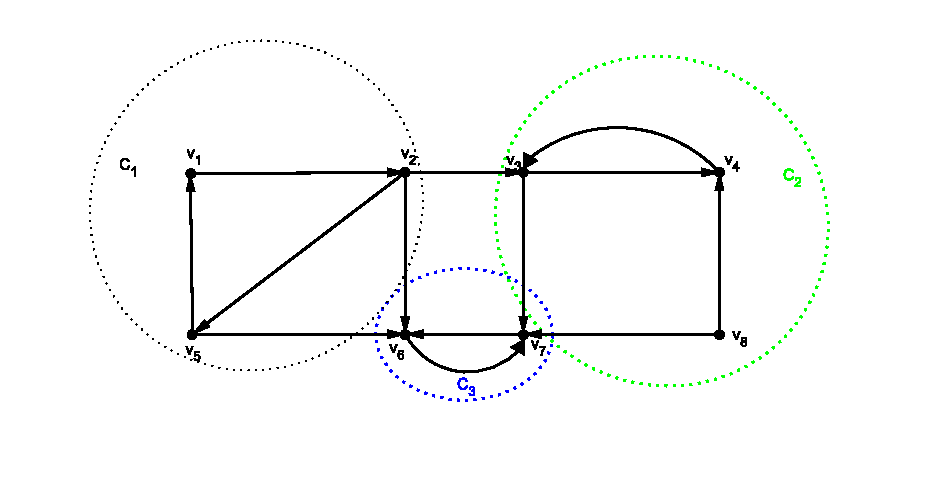
\includegraphics[scale=0.75]{componentes_conexa.eps}
\caption{$C_1$, $C_2$ y $C_3$ son componentes conexas de $D$}
\label{figura1}
\end{figure}


Una \emph{componente conexa} de una digr\'afica $D$ es una subdigr\'afica inducida maximal de $D$ que es fuertemente conexa. \\

%**************%**************%**********************%**********************%**************************

\chapter{Generalizaciones de n\'ucleos en digr\'aficas $m$-coloreadas con clases crom\'aticas cuasi-transitivas}

\section{La cerradura de una digr\'afica} 

Sea $D = (V,A)$ una digr\'afica $m$-coloreada. Definamos por $\mathcal{C}(D)$ a la digr\'afica cerradura de $D$. $\mathcal{C}(D)$ es tal que su conjunto de v\'ertices es el mismo que el de $D$ y tal que su conjunto de flechas, adem\'as de contener las mismas flecahs que $D$, por cada trayectoria monocrom\'atica en $D$ existe una flecha en $\mathcal{C}(D)$.

\begin{lemx}
Sea $D$ una digr\'afica m-coloreada. Si cada clase crom\'atica es cuasi-transitiva y sea $C_k$ un ciclo dirigido de longitud m\'inima en $Asym(\mathcal{C}(D))$. Existe un v\'ertice $u_i$ en $C_k$ en donde el ciclo tiene  cambio de color en las flechas de $C_k$ en alg\'un v\'ertice $u_i$ para alg\'un $i$ 
\end{lemx} 


\begin{proof}
Supongamos que el ciclo es monocrom\'atico. 
	\begin{figure} [ht!]
	\centering
	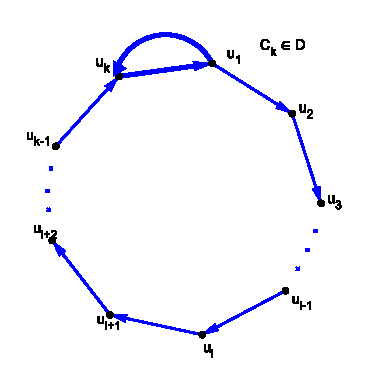
\includegraphics{figura1.eps}
	\caption{$C_k$ es un ciclo monocrom\'atico $D$}
	\label{figura1}
	\end{figure}
La $u_1u_k$-trayectoria monocrom\'atica $M = (u_1, u_2, \ldots, u_{k-1}, u_k)$ est\'a en $D$ ya que todas sus aristas est\'an en $C_k$. As\'i que la flecha $(u_1,u_k)$ est\'a en $\mathcal{C}(D)$. Sin embargo, la flecha $(u_k,u_1)$ en $C_k$ est\'a en $D$. Por lo tanto la flecha entre $u_k$ y $u_1$ es sim\'etrica. Luego, $(u_k,u_1)$ no es flecha de $C_k$, lo que contradice nuestra hip\'otesis inicial. 
\end{proof} 

\begin{lemx}
Sea $D$ una digr\'afica m-coloreada. Supongamos que cada clase crom\'atica en $D$ es cuasi-transitiva. Si $C_k$ es un ciclo dirigido en ${Asym(\mathcal{C}(D)}$, entonces $C_k$ es un ciclo dirigido en \emph{Asym(D)}. 	
\end{lemx}

\begin{proof}
Sea $C_k = (x_1, x_2, \ldots, x_{k-1})$ un ciclo dirigido asim\'etrico en la cerradura de $D$. Debido al resultado probado en el lema 2.1, sabemos que existe al menos una flecha en $C_k$ que sea de distinto color que las dem\'as. Supongamos que la flecha en donde $C_k$ cambia de color es $a=(x_i,x_{i+1})$. El caso en el que todas las flechas de $C_k$ est\'an en $D$ no necesita explicaci\'on, as\'i que supongamos que existe una flecha $a$ en $C_k$ que no es flecha de $D$. Si $a$ no es flecha de $D$, debe existir en $D$ una $x_{i}x_{i+1}-$trayectoria monocrom\'atica. Recordemos que esta flecha es asim\'etrica ya que $C_k$ es un ciclo asim\'etrico.
	\begin{figure} [ht!]
	\centering
	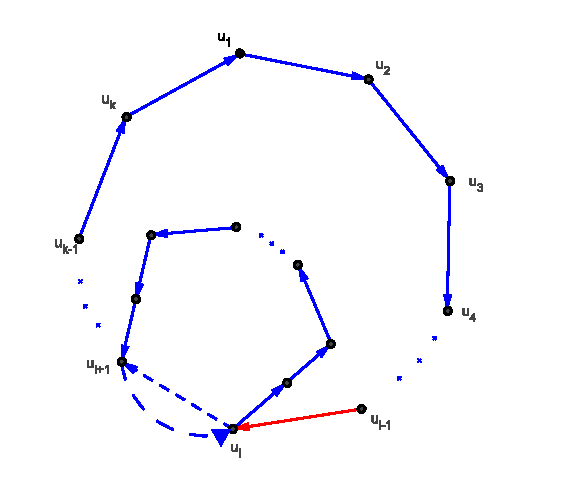
\includegraphics[scale=0.75]{c_k_2.eps}
	\caption{$C_k$ est\'a en $D$}
	\label{figura1}
	\end{figure}
Sea $P$ la $x_{i}x_{i+1}$-trayectoria monocrom\'atica en $D$ que da lugar a la existencia de $a$ en $\mathcal{C}(D)$. Supongamos que $P$ es minimal. Por hip\'otesis, cada clase crom\'atica en $D$ es cuasi-transitiva, y como $P$ es monocrom\'atica, podemos utilizar el resultado de la Proposici\'on 1.1. Notemos que, aunque $a$ es una flecha en $\mathcal{C}(D)$, hemos supuesto que $a$ no es una flecha de $D$. As\'i que descartamos el caso en el que la gr\'afica inducida de $P$ es semi-completa, ya que por ser $C_k$ un ciclo asim\'etrico, y $a$ una flecha en $C_k$, es imposible que exista la flecha $a' = (x_{i+1},x_i)$ en $D$, porque existir\'ia en $\mathcal{C}(D)$, haciendo sim\'etrica a $a$.
	\begin{figure} [ht!]
	\centering
	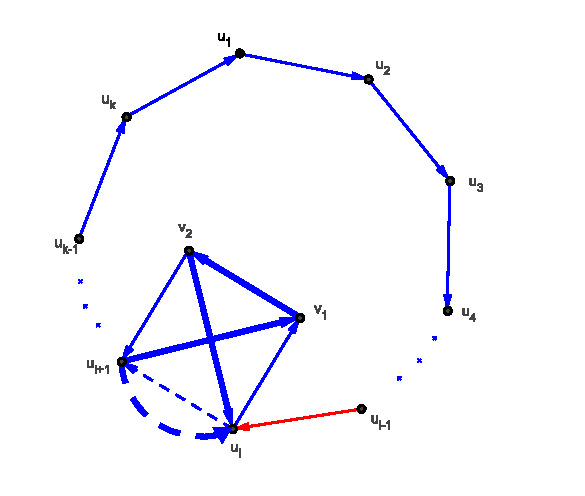
\includegraphics[scale=0.75]{c_k_3.eps}
	\caption{$C_k$ est\'a en $D$}
	\label{figura1}
	\end{figure}
Entonces el orden de $P$ debe ser 4. Deben existir, dos v\'ertices $v_1,v_2$, distintos de $x_i$ y $x_{i+1}$ en $D$, tales que $(x_{i+1},v,u,x_i)$ es una trayectoria monocrom\'atica del mismo color que $P$. La trayectoria $(x_{i+1}, v_2, v_1, x_i)$ de longitud 2 est\'a en $D$, as\'i que existe en $\mathcal{C}(D)$ la flecha $a'=(x_{i+1},x_i)$. Esto hace a la flecha $a$, que pertenece al ciclo asim\'etrico $C_k$, sim\'etrica, lo cual es imposible. 

Por lo tanto, no es posible que exista una flecha en $C_k$ que no est\'e en $D$ como quer\'iamos probar. 
\end{proof}

\section{N\'ucleos por trayectorias monocrom\'aticas} 

El concepto de n\'ucleo de una digr\'afica se defini\'o en el cap\'itulo 1. Esta definici\'on utiliza los conceptos de dominaci\'on e independencia de un subconjunto de v\'ertices de una digr\'afica. Podemos hacer la siguiente generalizaci\'on por trayectorias monocrom\'aticas: \\ 

Sea $D = (V, A)$ una digr\'afica. Sea $K \subset V$. Decimos que $K$ es un \emph{conjunto independiente por trayectorias monocrom\'aticas} de V, si para cualesquiera $u,v\in K$ no existe ninguna trayectoria entre $uv-$trayectoria monocrom\'atica en $D$. Decimos que un v\'ertice $v$ domina a un v\'ertice $x$ por trayectorias monocrom\'aticas si existe una $xv$-trayectoria monocrom\'atica en $D$. \\

Si para cada v\'ertice $x$ en $D$ que no est\'a en $K$ existe un v\'ertice $v$ en $K$ tal que $v$ domina a $x$ por trayectorias monocrom\'aticas, decimos que $K$ es un \emph{conjunto dominante por trayectorias monocrom\'aticas} de $V$. Si $K$ es independiente por trayectorias monocrom\'aticas y dominante por trayectorias monocrom\'aticas decimos que $K$ es un \emph{n\'ucleo} de $D$.

\begin{teox}
Si cada ciclo dirigido de una digr\'afica $D$ tiene una flecha sim\'etrica, entonces $D$ es kernel-pefecta.
\end{teox} 

\begin{lemx}
$K$ es un conjunto independiente en $\mathcal{C}(D)$ si y s\'olo si $K$ es un conjunto independiente por trayectorias monocrom\'aticas en $D$. 
\end{lemx}

\begin{proof}
Sean $u$ y $v$ dos v\'ertices en $K$. Supongamos que $K$ es un conjunto independiente en $\mathcal{C}(D)$ y que $P$ una $uv-$trayectoria monocrom\'atica en $D$. Si el orden de $P$ es 1, osea, $(u,v)$ est\'a en $D$, entonces lo est\'a en $\mathcal{C}(D)$, pero esto es imposible debido a la independencia de $K$. Si $P$ es una trayectoria monocrom\'atica de orden mayor a 1, tiene que existir una flecha $(u,v)$ en $\mathcal{C}(D)$ otra vez contradiciendo la independencia de $K$. Por lo tanto K es independiente por trayectorias monocrom\'aticas en $\mathcal{C}(D)$. \\

Ahora supongamos que $K$ es independiente por trayectorias monocrom\'aticas en $D$ y que $(u,v)$ es una flecha en $\mathcal{C}(D)$. Entonces $(u,v)$ es una flecha en $D$ (recordemos que una flecha es una trayectoria monocrom\'atica de longitud1), o bien, existe una $uv-$trayectoria monocrom\'atica, de orden mayor a 1, en $D$. contradiciendo la independencia por trayectorias monocrom\'aticas de $K$. Por lo tanto $K$ es independiente en $D$.
\end{proof} 

\begin{lemx}
$K$ es un conjunto dominante en $\mathcal{C}(D)$ si y s\'olo si $K$ es un conjunto dominante por trayectorias monocrom\'aticas en $D$.
\end{lemx}

\begin{proof}
Sean $x$ un v\'ertice en $D$ que no est\'e en $K$. Supongamos que $K$ es un conjunto dominante en $\mathcal{C}(D)$. Existe un v\'ertice $v$ en $K$ tal que la flecha $(v,x)$ est\'a en $\mathcal{C}(D)$. $v$ domina a $x$ por trayectorias monocrom\'aticas: si $(v,x)$ fuera flecha de $D$, ser\'ia una trayectoria monocrom\'atica de longitud 1. Si $(x,v)$ no fuera flecha de $D$, existir\'ia una $xv-$trayectoria monocrom\'atica en $D$. \\ 

Ahora supongamos que $K$ es un conjunto dominante por trayectorias monocrom\'aticas en $D$. Existe un v\'ertice $v$ en $K$ tal que existe una $vx$-trayectoria monocrom\'atica en $D$. Entonces existe la flecha $(v,x)$ en $\mathcal{C}(D)$, y por lo tanto $v$ domina a x. 
\end{proof}

\begin{teox} 
$K$ es un n\'ucleo en $\mathcal{C}(D)$ si y s\'olo si $K$ es un n\'ucleo por trayectorias monocrom\'aticas en $D$. 
\end{teox}
\begin{proof}
De los Lemas 2.4 y 2.5 se deduce este resultado 
\end{proof}


\section{Resultados}

%Las hip\'otesis de las que vamos a partir en la mayor\'ia de las demostraciones siguientes son sobre $D$. Los resultados que hemos probado anteriormente, en particular los lemas 2.1 y 2.6, no son ciertos necesariamente para $\mathcal{C}(D)$ aunque lo sean para $D$.\\

\begin{lemx}
Sea $D$ una digr\'afica m-coloreada tal que todas sus clases crom\'aticas son cuasi-transitivas. Si $C_k$ es un ciclo asim\'etrico dirigido de longitud m\'inima en $\mathcal{C}(D)$ cuasi-transitivo en el borde y $u_i$ es un v\'ertice en donde $C_k$ tiene un cambio de color en sus flechas, entonces $(u_{i+1},u_{i-1})$ no es flecha de $D$ y $(u_{i-1},u_{i+1})$ es flecha de $D$. 
\end{lemx} 

\begin{proof}
Sea $C_k = (u_0,u_1,\ldots,u_{k-1},u_0)$ un ciclo asim\'etrico en $\mathcal{C}(D)$. Debido al lema 2.1 sabemos que existe un v\'ertice en $C_k$, digamos $u_i$, tal que el ciclo cambia de color. Supongamos que las flechas distintas a $(u_i, u_{i+1})$ en $C_k$ son de color Azul, y la flecha $(u_i,u_{i+1})$ es de color Rojo. \\

	\begin{figure} [ht]
	\centering
	\includegraphics[scale=0.75]{C_k_changes_color.eps}
	\caption{$C_k$ tiene un cambio en el color de sus flechas en un v\'ertice $u_i$}
	\label{figura1}
	\end{figure}

Notemos que en virtud del lema 2.6, $C_k$ es un ciclo en $Asym(D)$.  $(u_{i-1}, u_i, u_{i+1})$ es una trayectoria monocrom\'atica en $C_k$, que es cuasi-transitivo en el borde por hip\'otesis, entonces alguna de las flechas $(u_{i-1},u_{i+1})$ o $(u_{i+1},u_{i-1})$ est\'a en $A(D)$. \\

Supongamos que es $a=(u_{i+1}, u_{i-1})$ la flecha en $A(D)$. En $D$ no hay tri\'angulos policrom\'aticos por hip\'otesis. $(u_i, u_{i+1})$ es una flecha roja y $(u_{i-1},u_i)$ es una flecha azul. Si $a$ fuera de color verde,  el tri\'angulo $(u_i,u_{i-1},u_{i+1},u_i)$ en $D$ tendr\'ia sus tres flechas de colores distintos, osea, ser\'ia policrom\'atico. Por lo tanto, $a$ solo puede estar en la clase crom\'atica Azul o en la clase crom\'atica Roja. \\

\begin{figure} [ht!]
    \begin{minipage}[b]{0.5\linewidth}
	\centering
	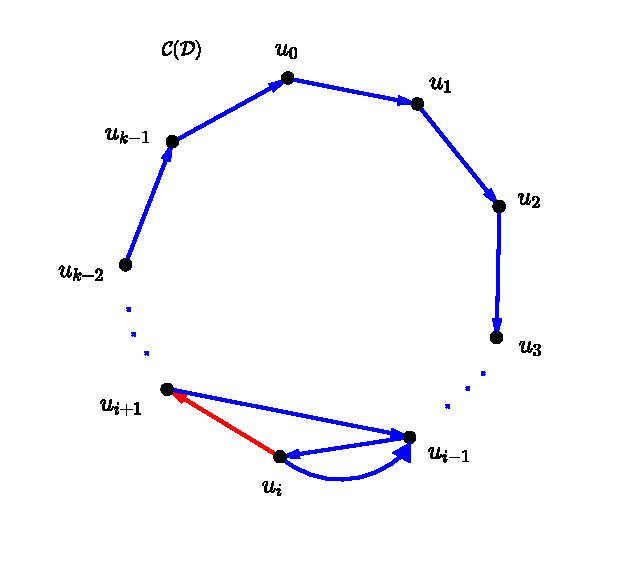
\includegraphics[scale=0.75]{u_i-1u_i+1_D_blue.eps}
	\caption{La flecha entre $u_{i-1}$ y $u_{i+1}$ es sim\'etrica en $D$}
	\label{figura2}
	\end{minipage}
	\hspace{0.5cm}
	\begin{minipage}[b]{0.5\linewidth}
   	\centering
	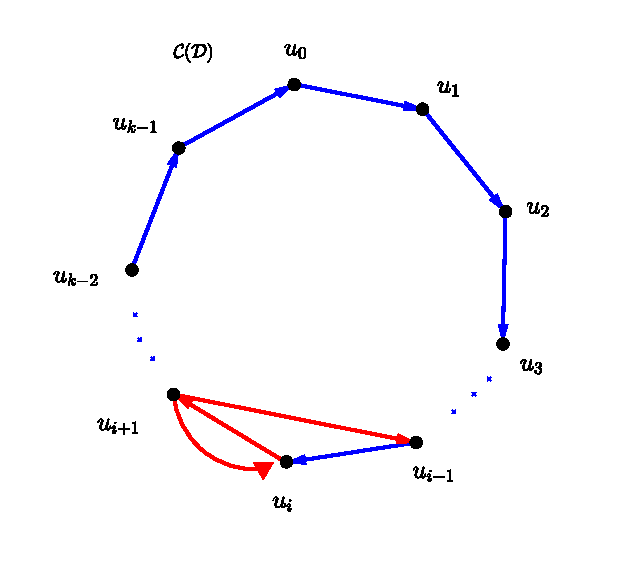
\includegraphics[scale=0.75]{u_i-1u_i+1_D_red.eps}
	\caption{La flecha entre $u_{i+1}$ y $u_i$ es sim\'etrica en $D$}
	\label{figura3}
    	\end{minipage}
\end{figure}

Supongamos que $a$ es una flecha de la clase crom\'atica Azul. La trayectoria monocrom\'atica $(u_{i+1},u_{i-1},u_i)$ est\'a en $D$, as\'i que $(u_{i+1},u_i)$ est\'a en $\mathcal{C}(D)$, ya que todas las clases crom\'aticas son cuasi-transitivas. Entonces la flecha entre $u_i$ y $u_{i+1}$ es sim\'etrica y por lo tanto $(u_i,u_{i+1})$ no est\'a en $C_k$. Esto es una contradicci\'on. \\ 

An\'alogamente, si $a$ fuera una flecha en la clase crom\'atica Roja, y como la trayectoria de longitud 2 monocrom\'atica roja $(u_{i-1},u_{i+1},u_i)$ est\'a en $D$, $(u_{i-1},u_i)$ est\'a en $\mathcal{C}(D)$. La flecha entre $u_{i-1}$ y $u_i$ es sim\'etrica y por lo tanto $(u_{i-1},u_i)$ no est\'a en el ciclo asim\'etrico $C_k$. Con esto descartamos tambi\'en la posibildiad de que $a$ sea una flecha en la clase crom\'atica Roja. \\ 

Hemos probado que la flecha en $D$ $a$  no puede ser de color azul ni rojo ni de ning\'un otro color distinto a estos dos, por lo tanto $a$ no puede estar en $D$, para futuras referencias notemos que esto no significa que $a$ no pueda estar en $\mathcal{C}(D)$. Por lo tanto, $a'=(u_{i-1},u_{i+1})$ debe estar en $D$. 


\end{proof}

\begin{lemx} 
Sea $D$ una digr\'afica m-coloreada sin tri\'angulos policrom\'aticos y con todas sus clase crom\'aticas cuasi-transitivas. Si $C_k$ es un ciclo asim\'etrico en $D$, cuasi-transitivo en el borde de longitud m\'inima y $u_i$ es un v\'ertice en $C_K$ en donde hay un cambio en el color en sus flechas, entonces existe una $u_{i+1}u_{i-1}$-trayectoria monocrom\'atica en $D$ que es de un color diferente al de $(u_i,u_{i+1})$ y al de $(u_{i-1},u_i)$.
\end{lemx} 

\begin{proof}
Sea $C_k$ es un ciclo asim\'etrico de longitud m\'inima. Probamos en el lema anterior que $(u_{i-1},u_{i+1})$ es una flecha en $D$ y por lo tanto es una flecha en $\mathcal{C}(D)$. El ciclo $C_{k-1} = (u_0,u_1,\ldots,u_{i-1},u_{i+1},\ldots,u_{k-1},u_k)$  tiene longitud menor que $C_k$, esto es imposible, porque por hip\'otesis $C_k$ es un ciclo m\'inimo en $Asym(\mathcal{C}(D)$.\\

\begin{figure} [ht!]
    \begin{minipage}[b]{0.5\linewidth}
	\centering
	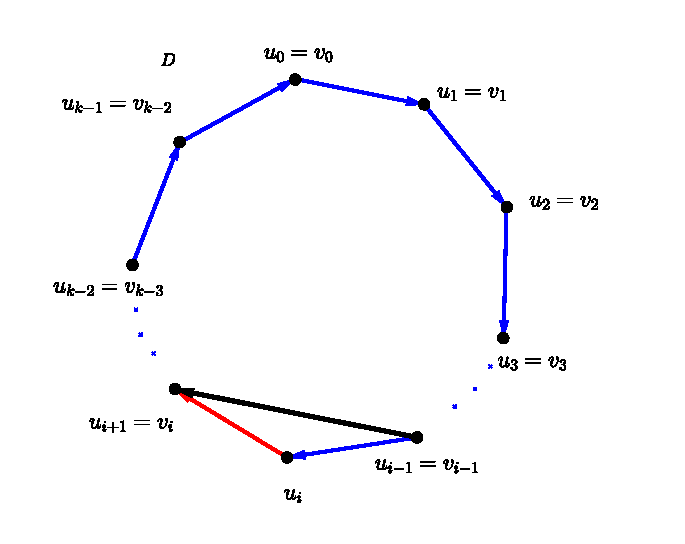
\includegraphics[scale=0.75]{arrow_in_D_C_k.eps}
	\caption{La flecha $(u_{i-1},u_{i+1})$ es parte de $C_{k-1}$ en $D$}
	\label{figura2}
	\end{minipage}
	\hspace{0.5cm}
	\begin{minipage}[b]{0.5\linewidth}
   	\centering
	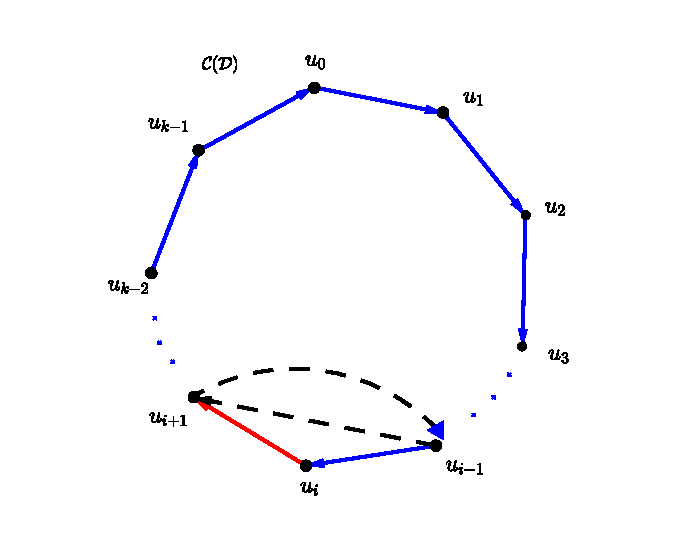
\includegraphics[scale=0.75]{symmetric_arrow_in_C_k.eps}
	\caption{La flecha entre $u_{i+1}$ y $u_i$ debe ser sim\'etrica en $D$}
	\label{figura3}
    \end{minipage}
\end{figure}

Entonces la flecha entre $u_{i-1}$ y $u_{i+1}$ es sim\'etrica en $\mathcal{C}(D)$, y por lo tanto no est\'a en $Asym(\mathcal{C}(D)$. Osea, las flechas $a$ y $a'$ est\'an en $\mathcal{C}(D)$. Como ya probamos que $a = (u_{i+1},u_{i-1})$ no es una flecha de $D$, debe existir una $u_{i+1}u_{i-1}-$trayectoria monocrom\'atica en $D$.  
\begin{figure} [ht!]
	\centering
	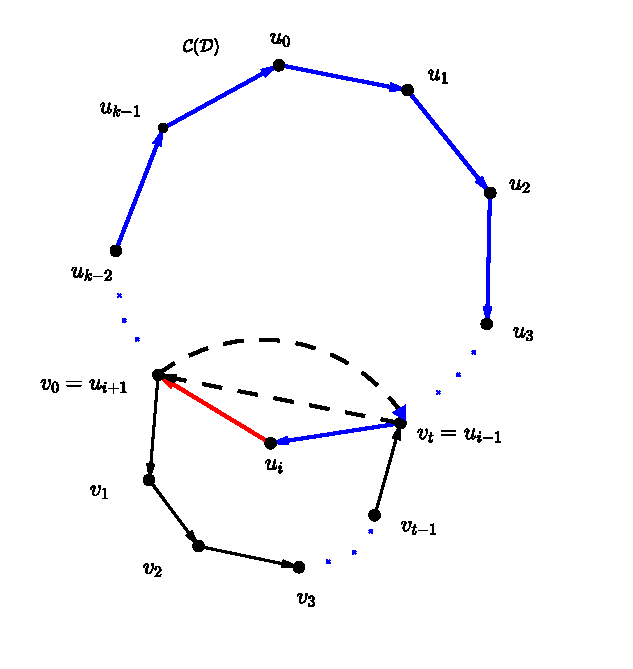
\includegraphics[scale=0.75]{P_is_in_D_1.eps}
	\caption{Existe una $u_{i-1}$$u_{i+1}$-trayectoria monocrom\'atica en $D$}
	\label{figura2}
\end{figure}
Llamemos $P$ a esta trayectoria. $P$ es del mismo color que $(u_{i+1},u_{i-1})$ y tiene que ser distinto de Rojo o Azul:\\

\begin{figure} [ht!]
    \begin{minipage}[b]{0.5\linewidth}
	\centering
	\includegraphics[scale=0.75]{P_is_blue.eps}
	\caption{Si $P$ es roja, la flecha entre $u_i$ y $u_{i+1}$ es sim\'etrica en $\mathcal{C}(D)$}
	\label{figura2}
	\end{minipage}
	\hspace{0.5cm}
	\begin{minipage}[b]{0.5\linewidth}
   	\centering
	\includegraphics[scale=0.75]{P_is_red.eps}
	\caption{Si $P$ es azul, la flecha entre $(u_{i-1}$ y $u_i$ es sim\'etrica en $\mathcal{C}(D)$}
	\label{figura3}
    \end{minipage}
\end{figure}
Si $(u_{i+1},u_{i-1})$ fuera Azul, la $u_{i-1}u_i$-trayectoria Azul se forma en $D$, y por ende la flecha $(u_{i+1},u_i)$ est\'a en $\mathcal{C}(D)$, ya que cada clase crom\'atica es cuasi-transitiva. La flecha $(u_i,u_{i+1})$ tambi\'en est\'a en $\mathcal{C}(D)$ pues es una flecha de $C_k$. Por lo tanto la flecha entre $u_i$ y $u_{i+1}$ es sim\'etrica, pero esto es imposible ya que supusimos que $(u_i,u_{i+1})$ est\'a en $C_k$, un ciclo asim\'etrico.
Si esta flecha fuera Roja, haciendo un an\'alisis similar al anterior, tendr\'iamos la trayectoria monocrom\'atica $(u_i,u_{i+1},\ldots,u_{i-1})$ de color Rojo, luego, $(u_i,u_{i-1})$ es una flecha en $\mathcal{C}(D)$, entonces la flecha entre $u_{i-1}$ y $u_i$, ambos v\'ertices en $C_k$, es sim\'etrica en $\mathcal{C}(D)$, lo que contradice la asimetricidad de $C_k$.
\end{proof}

\begin{lemx}
Sea $D$ es una digr\'afica con cada clase crom\'atica cuasi-transitiva, sin tri\'angulos policrom\'aticos. Si $P$ es una $u_{i+1}u_{i-1})$ trayectoria moncorom\'atica en $D$, el v\'ertice $u_i$ no forma parte de la $u_{i+1}u_i$-trayectoria verde en $D$. 
\end{lemx}

\begin{proof}
Sea $P$ la $u_{i+1}u_i$-trayectoria en $D$ que existe en virtud del Lema 2.9. Supongamos que  $u_i$ es un v\'ertice $v_k$ de la trayectoria verde $P$:  \\
\begin{figure} [ht!]
\centering
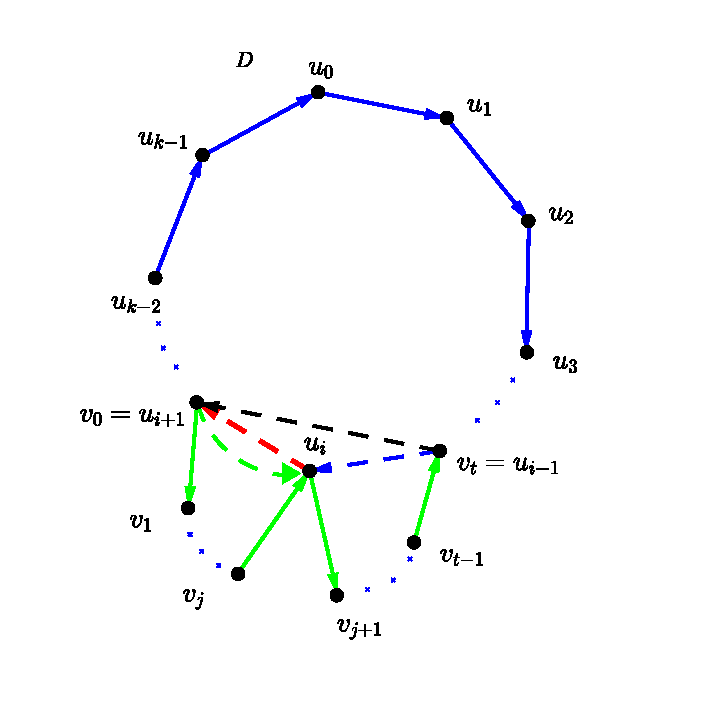
\includegraphics[scale=0.75]{ui_not_in_P.eps}
\caption{$u_i$ no es v\'ertice de $P$}
\label{figura1}
\end{figure}

Entonces la flecha $(u_{i+1},u_i)$ est\'a en $\mathcal{C}(D)$. La flecha $(u_i, u_{i+1})$ no est\'a en $C_k$, porque es sim\'etrica. Esto es una contradicci\'on. Por lo tanto $u_i$ no es un v\'ertice en $P$. 
\end{proof}

\begin{teox} Sea $D  = (V,F)$ una digr\'afica m-coloreada sin tri\'angulos policrom\'aticos y con todas sus clases crom\'aticas cuasi-transitivas. Supongamos que $C_k \in D$ es un ciclo cuasi-transitivo en el borde de longitud m\'inima. Entonces: \\

1) Existe un v\'ertice $u_i$ en $C_k$, tal que todas las flechas en el ciclo son de color Azul y $(u_i,u_{i+1})$ es de color Rojo 

2) $(u_{i-1}, u_{i+1})$ est\'a en $D$ 

3) $(u_{i+1},u_{i-1})$ no es una flecha en $D$, $(u_{i+1},u_{i-1})$ si una flecha en $\mathcal{C}(D)$, y por lo tanto existe $P$, una $u_{i+1}u_{i-1}-$trayectoria en $D$, de color Verde 

4) $u_i$ no es un v\'ertice de $P$ 
\end{teox}

\begin{teox}
Sea $D = (V,F)$ una digr\'afica m-coloreada sin tri\'angulos policrom\'aticos y con todas sus clases crom\'aticas cuasi-transitivas. Supongamos que cada ciclo en $D$ es cuasi-transitivo en el borde. Si $C_k$ es un ciclo asim\'etrico de longitud m\'inima en $D$, entonces $C_k$ tiene una flecha sim\'etrica.  
\end{teox}

\begin{proof}
	Sea $C_k = (u_1,u_2,\ldots,u_{k-1},u_0)$ un ciclo dirigido en $Asym(\mathcal{C}(D))$. Son v\'alidas todas las hip\'otesis sobre $C_k$ que nos garantizan el resultado probado en el Teorema 2.10. Entonces, existe en $D$ una $u_{i+1}u_{i-1}$-trayectoria monocrom\'atica, $P$, de color Verde en y el v\'ertice $u_i$ no forma parte de $P$. Supongamos sin p\'erdida de generalidad que $P$ es de longitud m\'inima.
$P$ es una $u_{i+1}u_{i-1}$-trayectoria en la clase crom\'atica del Verde, sin embargo, la flecha $(u_{i-1},u_{i+1})$ no lo est\'a. Las flechas $(u_{i-1},u_i)$ y $(u_i,u_{i+1})$ son de distintos colores ya que en $u_i$ hay un cambio de color en el ciclo. Debido a esto la flecha $(u_{i-1},u_{i+1})$ no puede ser de color Verde debido a que en $D$ no hay tri\'angulos policrom\'aticos. 
La clase crom\'atica Verde contiene completamente a la trayectoria $P$, y como cada clase crom\'atica es cuasi-transitiva en $D$, podemos utilizar el resultado de la Proposici\'on 1.2, el cual garantiza que la longitud de $P$ es 4.
\begin{figure} 
\centering 
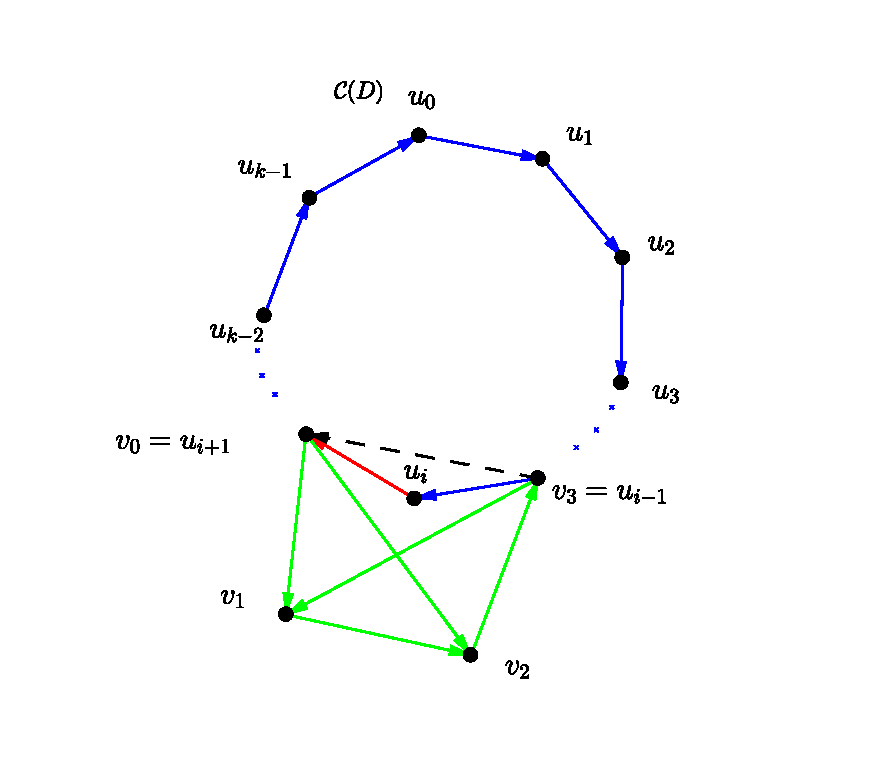
\includegraphics[scale=0.6]{P_has_order_4.eps}
\caption{El orden de $P$ es 4}
\label{figura1}
\end{figure}
Adem\'as existen v\'ertices, digamos $v_1$ y $v_2$, en la clase crom\'atica Verde de $D$, distintos a $u_{i+1}$ y a $u_{i-1})$, tales que las trayectorias dirigidas $(u_{i+1},v_2,v_1,u_{i-1})$ y $(u_{i-1},v_1,v_2,u_{i+1})$ tambi\'en est\'an en la clase crom\'atica Verde en $D$.\\ 

Estas flechas son parte del ciclo $(u_i,u_{i+1},v_1,v_2,u_{i-1},u_i)$. Como todos los ciclos en $D$, este es cuasi-trasntivio en el borde por hip\'otesis, as\'i que debe existir una flecha entre $u_i$ y $v_1$ en $D$, como consecuencia de que la trayectoria de longitud dos $(u_i,u_{i+1},v_1)$ est\'a en $D$. Digamos que $a = (u_i,v_1)$ y $a' = (v_1,u_i)$. \\ 

Supongamos que $a$ es la flecha que est\'a en $D$. Si fuera de color azul, el tri\'angulo $(u_i,u_{i+1},v_1)$ ser\'ia policrom\'atico en $D$: 

Si $a$ fuera de color rojo, el tri\'angulo $(u_i,v_1,u_{i-1})$ ser\'ia policrom\'atico 

\begin{figure} 
    \begin{minipage}[b]{0.5\linewidth}
	\centering
	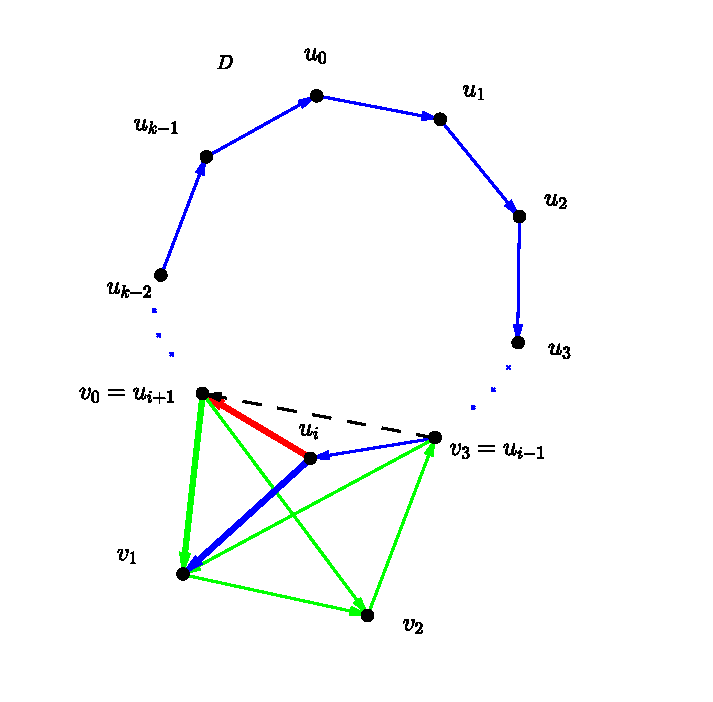
\includegraphics[scale=0.6]{a_is_blue.eps}
	\caption{El triangulo $(u_i,u_{i+1},v_1)$ es policrom\'atico}
	\label{figura2}
	\end{minipage}
	\hspace{0.5cm}
	\begin{minipage}[b]{0.5\linewidth}
   	\centering
	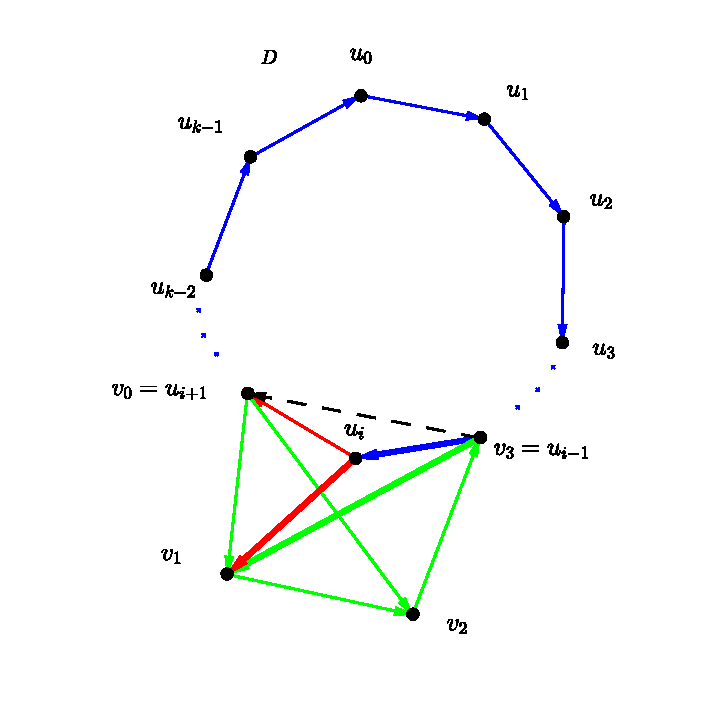
\includegraphics[scale=0.6]{a_is_red.eps}
	\caption{El triangulo $(u_i, v_1, u_{i-1})$ es policrom\'atico}
	\label{figura3}
    \end{minipage}
\end{figure}


Finalmente, si $a$ fuera de color verde, la flecha $(u_i,u_{i-1})$ est\'a en $\mathcal{C}(D)$ como consecuencia de la existencia de la trayectoria monocrom\'atica verde $(u_i, v_1, u_{i-1})$ en $D$, haciendo sim\'etrica la flecha formada por los v\'eritces $u_{i-1}$ y $u_i$, ambos en el ciclo asim\'etrico $C_k$, lo cual es imposible. \\ 

\begin{figure} [ht!]
\centering
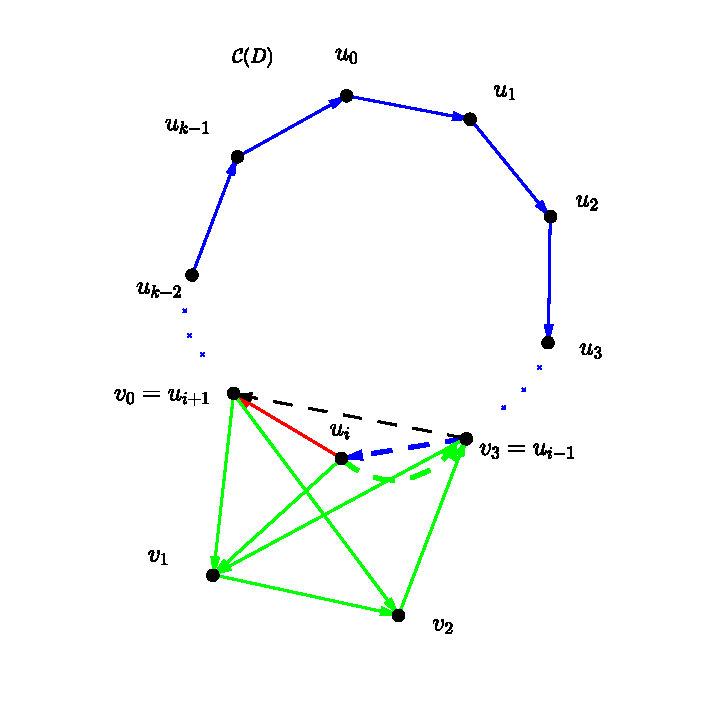
\includegraphics[scale=0.6]{a_is_green.eps}
\caption{La flecha entre $u_{i-1}$ y $u_i$ es sim\'etrica}
\label{figura1}
\end{figure}

Por lo tanto es imposible que $a$ sea una flecha en $D$. Supongamos ahora que $a'$ es la flecha que est\'a en $D$. \\

An\'alogamente al caso anterior, si $a'$ fuera Azul o Roja, los tri\'angulos $(u_i,u_{i+1},v_1)$ o $(u_i,v_1,u_{i-1})$ ser\'ian policrom\'aticos, contradiciendo nuestras hip\'otesis.

\begin{figure} [ht!]
    \begin{minipage}[b]{0.5\linewidth}
	\centering
	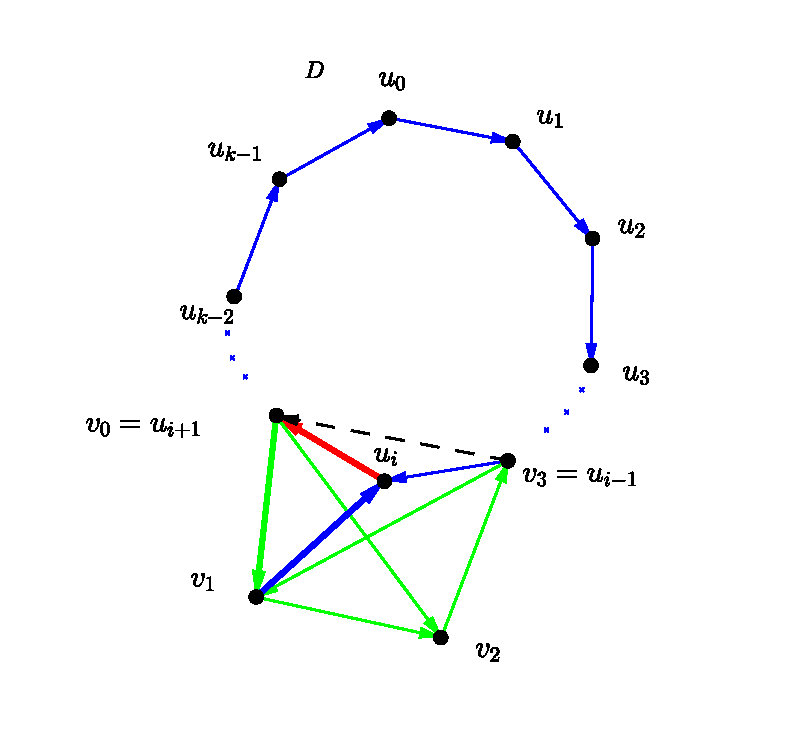
\includegraphics[scale=0.6]{aprime_is_blue.eps}
	\caption{El tri\'angulo $(u_i,u_{i+1},v_1)$ es policrom\'atico}
	\label{figura2}
	\end{minipage}
	\hspace{0.5cm}
	\begin{minipage}[b]{0.5\linewidth}
   	\centering
	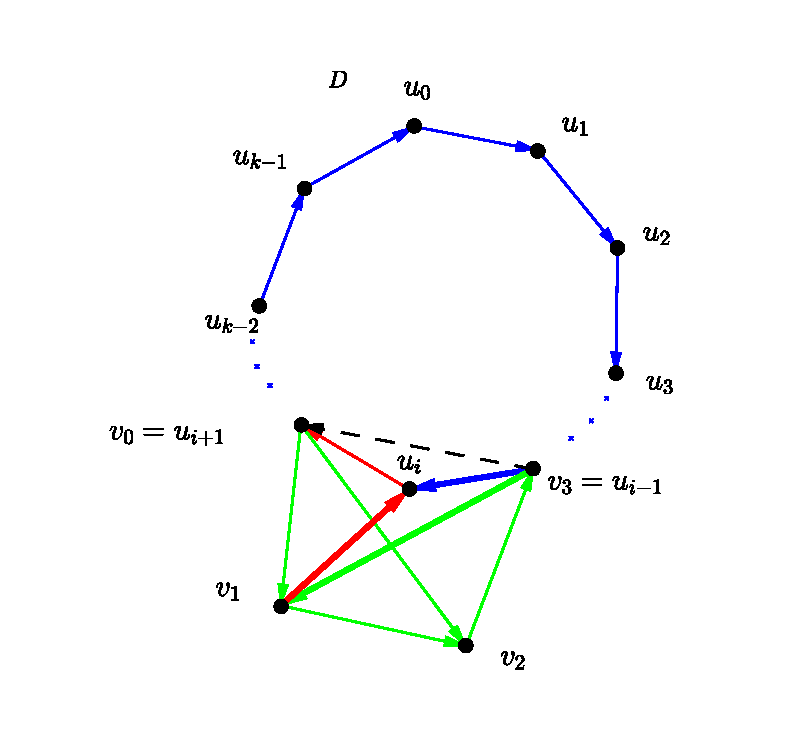
\includegraphics[scale=0.6]{aprime_is_red.eps}
	\caption{El tri\'angulo $(u_i,v_1,u_{i-1})$ es policrom\'atico}
	\label{figura3}
    \end{minipage}
\end{figure}

Igual que en el caso anterior, Si $a'$ fuera de color verde, la flecha entre $u_i$ y $u_{i+1}$ ser\'ia sim\'etrica, lo cual es imposible 

\begin{figure} [ht!]
\centering
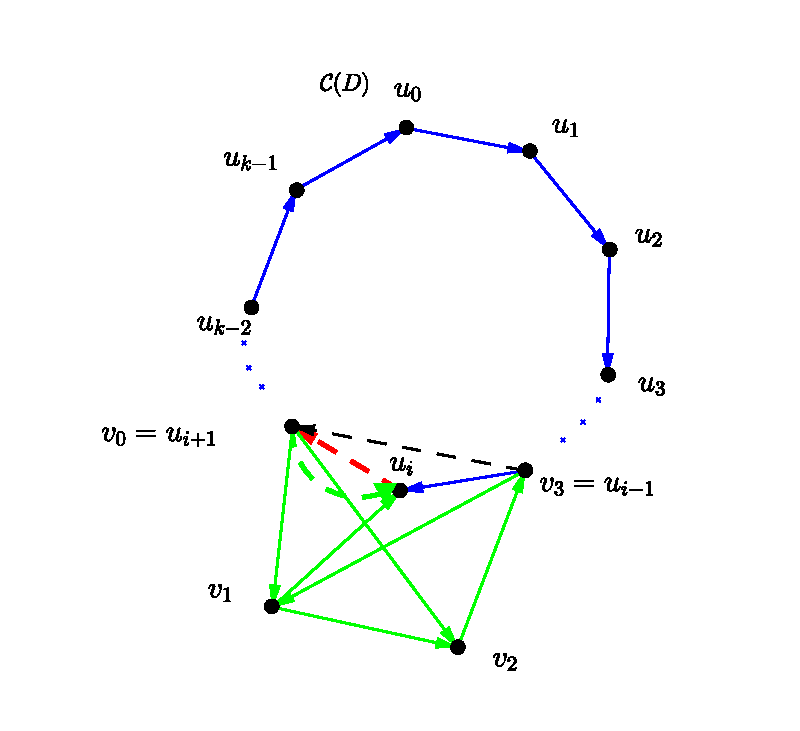
\includegraphics[scale=0.6]{aprime_is_green.eps}
\caption{La flecha entre $u_i$ y $u_{i+1}$ es sim\'etrica}
\label{figura1}
\end{figure}
\end{proof}

En la deomstraci\'on del Teorema 2.4, supusimos que la digr\'afica $D$ no contiene tri\'angulos policrom\'aticos. Esto incluye tanto a torneos $TT_3$ como a $C_3$, ciclos de tama\~no 3. En el siguiente Teorema vamos a cambiar esta hip\'otesis por una m\'as fuerte, permitiendo la existencia de torneos de 3 v\'ertices policrom\'aticos. En el caso de los ciclos de longitud 3, vamos a limitar la cantidad de aristas de distinto color a 2, permitiendo tri\'angulos casi-monocrom\'aticos pero no policrom\'aticos. \\

\begin{teox}
Sea $D$ una digr\'afica $m$-coloreada tal que cada ciclo es cuasi-transitivo en el borde y cada una de sus clases crom\'aticas es cuasi-transitiva. Si existen enteros $4 \leq k$ y $3 \leq l \leq k - 1$ tales que cada ciclo $C_k$ es casi-monocrom\'atico y cada $C_l$ no es policrom\'atico, entonces $D$ tiene un n\'ucleo por trayectorias monocrom\'aticas. 
\end{teox}
\begin{proof}
Sea $C_k = (u_1,u_2,\ldots,u_{k-2},u_{k-1},u_L)$ un ciclo dirigido \emph{asim\'etrico} de longitud m\'inima en $\mathcal{C}(D)$. Por hip\'otesis sabemos que cada $C_l$ no es policrom\'atico para $3 \leq l$, as\'i que se cumplen las hip\'otesis del Teorema 2.4 y podemos afirmar lo siguiente: La flecha $(u_{i-1},u_{i+1})$ est\'a en $D$, $(u_{i+1},u_{i-1})$ no est\'a en $D$ pero si est\'a en $\mathcal{C}(D)$, y debido a esto, existe $P$ una $u_{i+1}u_{i-1}-$trayectoria en $D$. Adem\'as $u_i$ no est\'a en $P$ \\

Supongamos que $(u_{i-1},u_{i+1})$ no est\'a en la clase crom\'atica Verde. Como todas las clases crom\'aticas en $D$ son cuasi-transitivas, el orden de $P$ es 4. El ciclo $C' = (u_i,u_{i+1},v_1,v_2,u_{i-1},u_i)$ est\'a en $D$, es policrom\'atico y tiene longitud 5. \\

\begin{figure} [ht!]
\centering
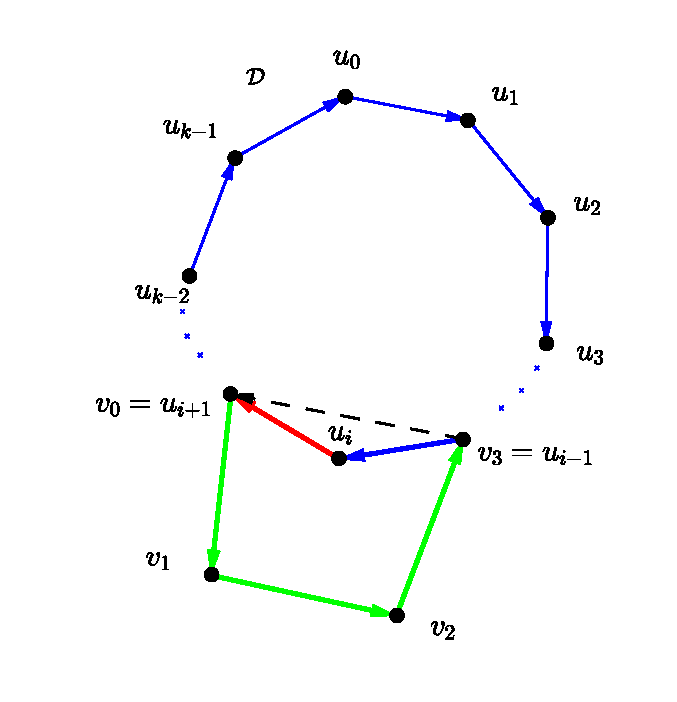
\includegraphics[scale=0.6]{C_5_policromatico.eps}
\caption{Un ciclo de longitud 5 policrom\'atico en $D$}
\label{figura1}
\end{figure}

Si $k$ fuera igual a 6 o mayor que 6, todos los ciclos de orden menor a 6 deben ser no policrom\'aticos por hip\'otesis, el orden de $C'$ es menor que 6, igual a 5, y es policrom\'atico. Entonces $k$ no puede ser mayor que 5.  \\

Adem\'as, si $k$ fuera 5, todos los ciclos de longitud 5 deber\'ian ser casi-monocrom\'aticos. Notemos que un ciclo policrom\'atico no es casi-monocrom\'atico, as\'i que el ciclo $C'$ policrom\'atico contradice nuestras hip\'otesis tambi\'en. Por lo tanto $k$ debe ser menor que 5. \\

Si $k$ es menor que 5, debe ser igual a 4. Como cada ciclo es cuasi-transitivo en el borde por hip\'otesis, una flecha entre los v\'ertices $u_i$ y $v_1$ debe estar en $D$, ya sea $(u_i,v_1)$ o $(v_1,u_i)$. \\

Supongamos que $(u_i,v_1)$ est\'a en $D$. Como cada $C_4$ es casi-monocrom\'atico $(u_i,v_1)$ debe ser Verde, de otra forma el ciclo de orden 4 $(u_i,v_1,v_2,u_{i-1},u_i)$ no es casi-monocrom\'atico, contendr\'ia dos flechas azules y dos verdes, o una flecha roja, una azul y dos verdes. \\

\begin{figure} [ht!]
    \begin{minipage}[b]{0.5\linewidth}
	\centering
	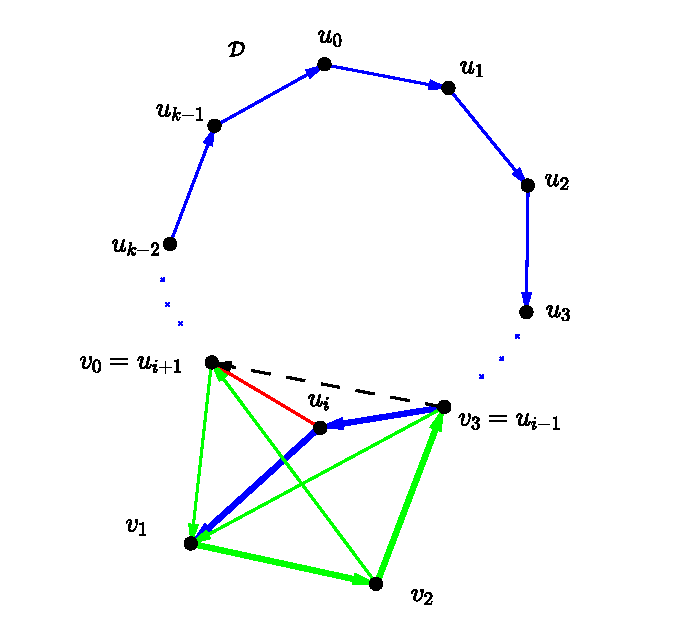
\includegraphics[scale=0.6]{C_4_policromatico_blue.eps}
	\caption{El ciclo $(u_i,v_1,v_2,u_{i-1},u_i)$ no es casi-monocrom\'atico}
	\label{figura2}
	\end{minipage}
	\hspace{0.5cm}
	\begin{minipage}[b]{0.5\linewidth}
   	\centering
	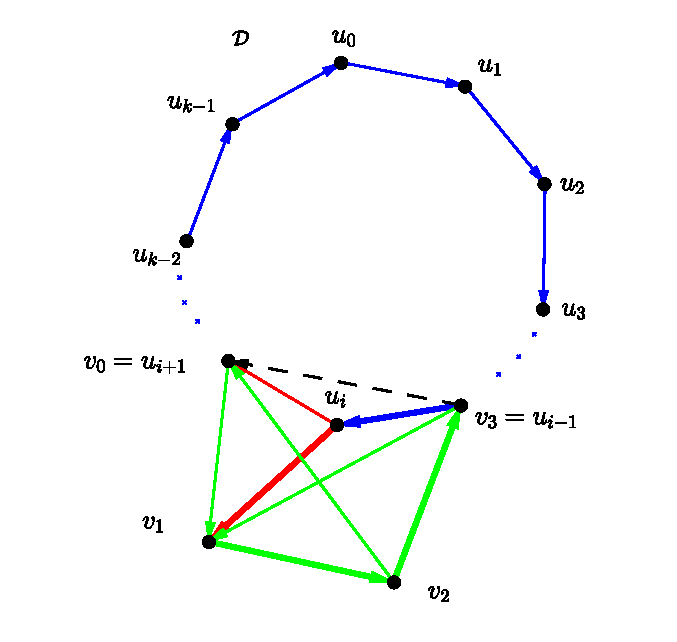
\includegraphics[scale=0.6]{C_4_policromatico_roja.eps}
	\caption{El ciclo $(u_i,v_1,v_2,u_{i-1},u_i)$ no es casi-moncorom\'atico}
	\label{figura3}
    \end{minipage}
\end{figure}

\begin{figure} [ht!]
\centering
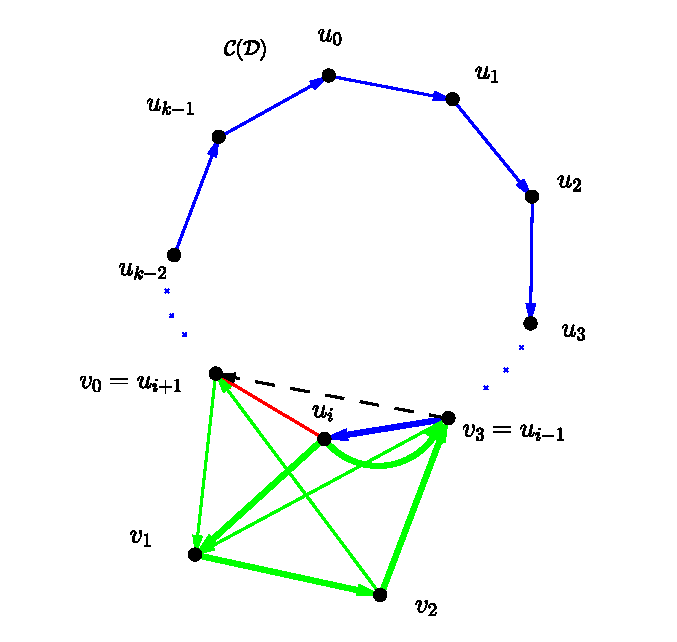
\includegraphics[scale=0.6]{C_4_casimonocromatico_verde.eps}
\caption{Si $(u_i,v_1)$ es Verde, la flecha sim\'etrica $(u_i,u_{i-1})$ est\'a en $\mathcal{C}(D)$}
\label{figura1}
\end{figure}

$(u_i,v_1)$ est\'a en la trayectoria moncorom\'atica $(u_i,v_1,v_2,u_{i-1})$ en $D$, lo que garantiza la existencia de $(u_i,u_{i-1})$ en $\mathcal{C}(D)$. Entonces, la flecha entre $u_i$ y $u_{i+1}$, que forma parte de $C_k$ es sim\'etrica en $\mathcal{C}(D)$, esto es imposible ya que $C_k$ es un ciclo asim\'etrico en $D$. \\

Entonces $(v_1,u_i)$ es flecha en $A(D)$. \\

Si $(v_1,u_i)$ estuviera en $D$ y fuera de color Azul, $(u_i,u_{i+1},v_1,u_i)$ ser\'ia un ciclo policrom\'atico de longitud 3 menor a $k$, lo que ser\'ia una contradicci\'on. 

Si $(v_1,u_i)$ fuera de color Verde, la $u_{i+1}u_i$-trayectoria verde da lugar a la flecha $(u_{i+1},u_i)$, haciendo la flecha entre estos dos v\'ertices sim\'etrica, lo que es imposible. \\ 

Por lo tanto $(v_1,u_i)$ es de color Rojo. \\ 

\begin{figure} [ht!]
    \begin{minipage}[b]{0.5\linewidth}
	\centering
	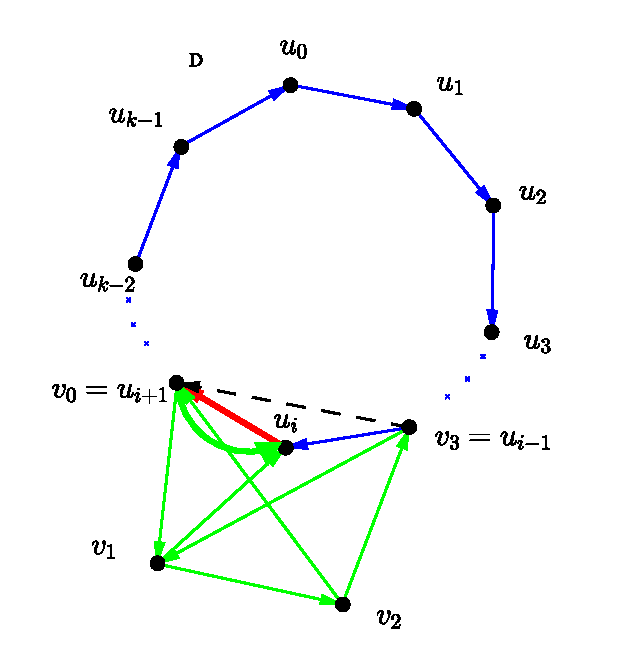
\includegraphics[scale=0.6]{v1_ui_green.eps}
	\caption{El ciclo $(u_i,v_1,v_2,u_{i-1})$ es policrom\'atico}
	\label{figura2}
	\end{minipage}
	\hspace{0.5cm}
	\begin{minipage}[b]{0.5\linewidth}
   	\centering
	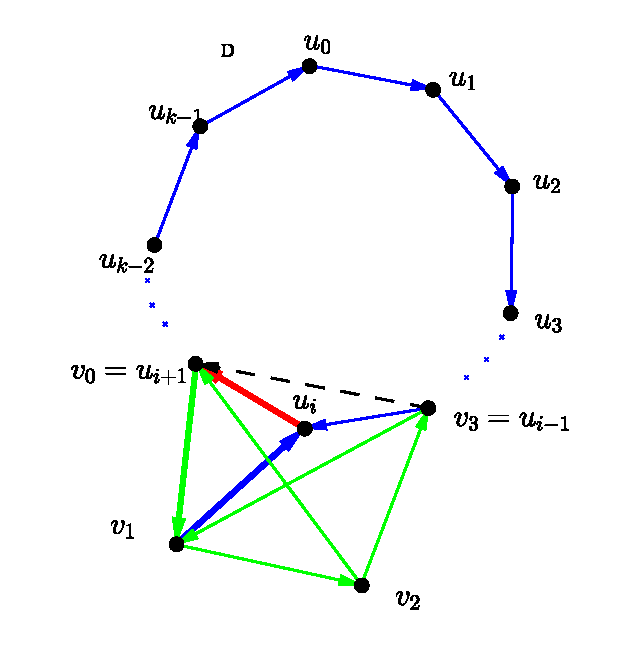
\includegraphics[scale=0.6]{v1_ui_blue.eps}
	\caption{El ciclo $(u_i,v_1,v_2,u_{i-1})$ es policrom\'atico}
	\label{figura3}
    \end{minipage}
\end{figure}


\begin{figure} [ht!]
\centering
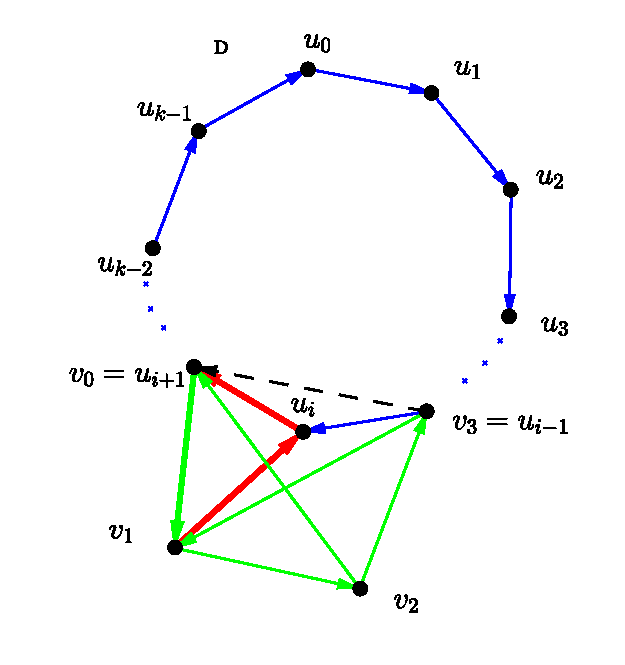
\includegraphics[scale=0.6]{v1_ui_red.eps}
\caption{Si $(u_i,v_1)$ es Verde, la flecha sim\'etrica $(u_i,u_{i-1})$ est\'a en $\mathcal{C}(D)$}
\label{figura1}
\end{figure}

La flecha entre $v_2$ y $u_i$ debe estar en $D$ como consecuencia de que la trayectoria $(v_2,u_{i-1},u_i)$ forma parte del ciclo $C_5$, cuasi-transitivo en el borde por hip\'otesis.\\

Supongamos que $(v_2,u_i)$ est\'a en $D$. Esta flecha solo puede ser Verde para que el ciclo de longitud 4 $(u_i,u_{i+1},v1,v2,u_i)$ sea casi-monocrom\'atico. La flecha $(u_{i+1},u_i)$ est\'a en $D$ como consecuencia de la $u_{i+1}u_i$-trayectoria monocrom\'atica Verde en $D$, haciendo sim\'etrica la flecha entre estos v\'ertices. \\

\begin{figure} [ht!]
    \begin{minipage}[b]{0.5\linewidth}
	\centering
	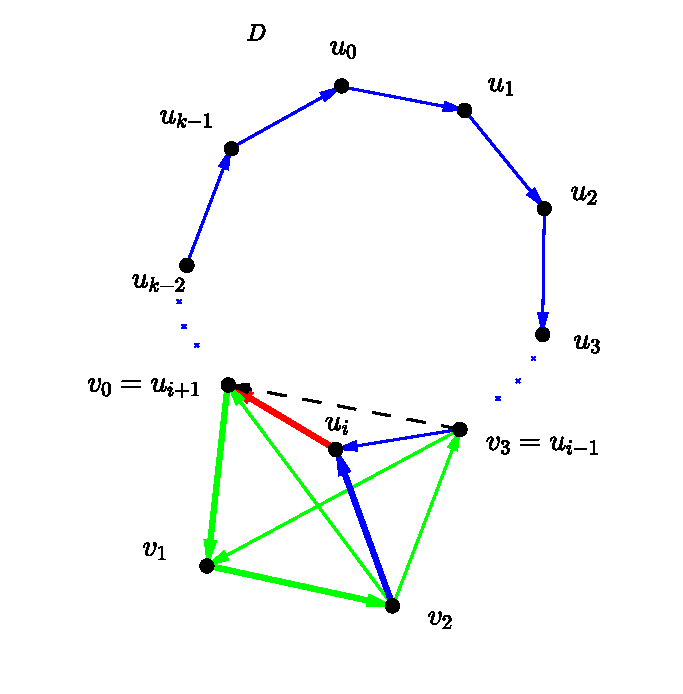
\includegraphics[scale=0.6]{v2_ui_blue.eps}
	\caption{El ciclo de orden 4 $(u_i,v_1,v_2,u_{i-1}, u_i)$ no es casi-monocrom\'atico}
	\end{minipage}
	\hspace{0.5cm}
	\begin{minipage}[b]{0.5\linewidth}
   	\centering
	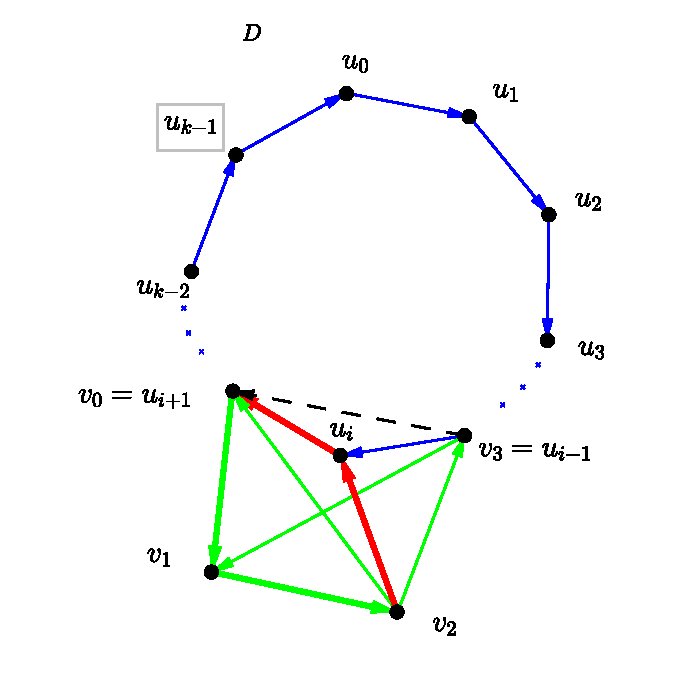
\includegraphics[scale=0.6]{v2_ui_red.eps}
	\caption{El ciclo de orden 4 $(u_i,v_1,v_2,u_{i-1},u_i) $no es casi-monocrom\'atico}
    \end{minipage}
\end{figure}

\begin{figure} [ht!]
\centering
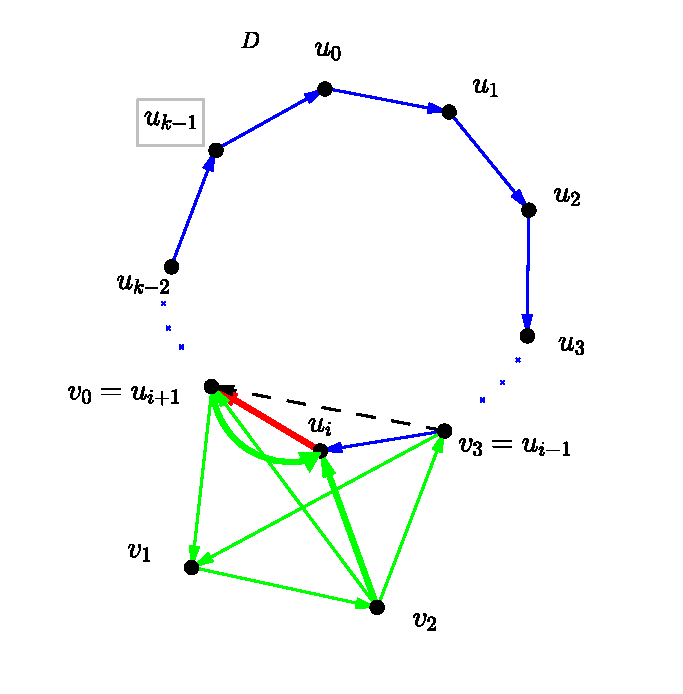
\includegraphics[scale=0.6]{v2_ui_green.eps}
\caption{Si $(v_2,u_i)$ es Verde, la flecha sim\'etrica $(u_i,u_{i+1})$ est\'a en $\mathcal{C}(D)$}
\label{figura1}
\end{figure}

Por lo tanto, $(u_i,v_2)$ debe estar en $D$. No puede ser Verde, porque la flecha entre $u_{i-1}$ y $u_i$ ser\'ia sim\'etrica, como consecuencia de la existencia de la trayectoria verde $(u_i,v_2,u_{i-1})$. Si fuera de color Rojo, el ciclo de orden 3 $(u_{i-1},u_i,v_2,u_{i-1})$ ser\'ia policrom\'atico, otra vez una contradicci\'on. 

\begin{figure} [ht!]
    \begin{minipage}[b]{0.5\linewidth}
	\centering
	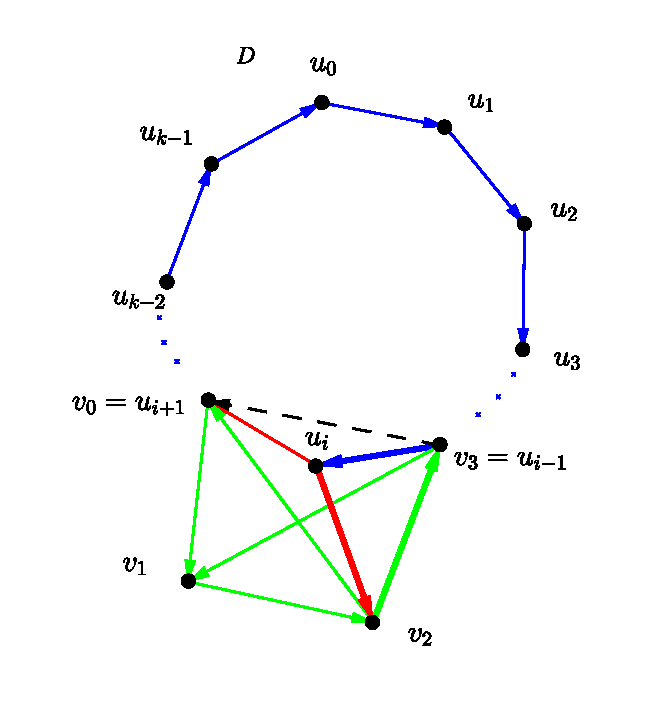
\includegraphics[scale=0.6]{ui_v2_red.eps}
	\caption{El ciclo de longitud 3 $(u_i,v_2,u_{i-1},u_i)$ es policrom\'atico}
	\end{minipage}
	\hspace{0.5cm}
	\begin{minipage}[b]{0.5\linewidth}
   	\centering
	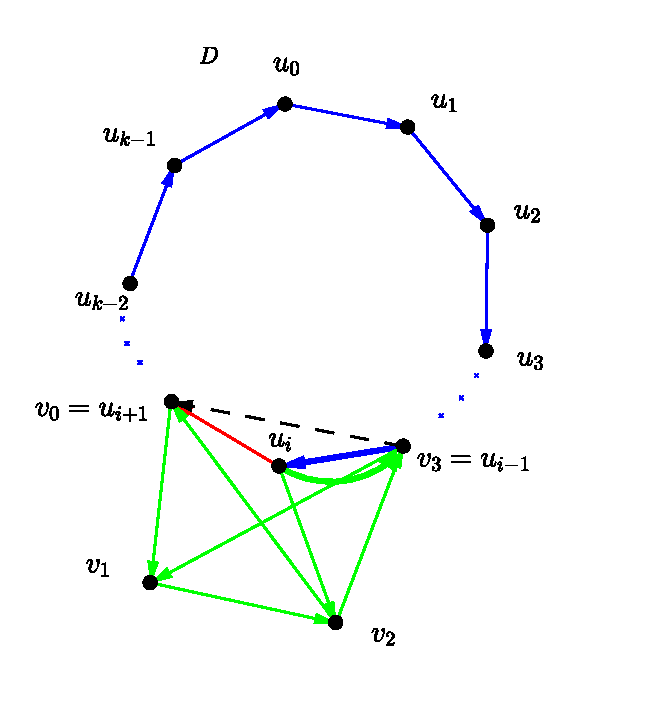
\includegraphics[scale=0.6]{ui_v2_green.eps}
	\caption{La flecha $(u_{i-1},u_i)$ en $C_k$ es sim\'etrica}
    \end{minipage}
\end{figure}

\begin{figure} [ht!]
\centering
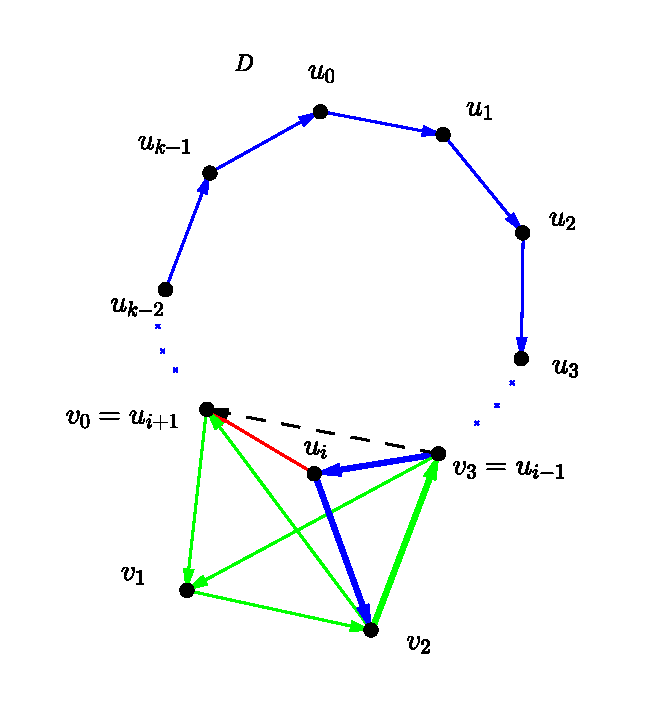
\includegraphics[scale=0.6]{ui_v2_blue.eps}
\caption{$(u_i,v_2)$ debe ser azul}
\label{figura1}
\end{figure}

%Por lo tanto $(u_{i-1},u_{i+1})$ es Verde. 

%En este caso, la flecha $(u_{i-1},u_{i+1})$ podr\'ia ser de color Verde sin contradecir nuestras hip\'otesis sobre la coloraci\'on de $D$, ya que $D$ admite torneos $TT_3$ policrom\'aticos. 

%$(u_{i-1},u_{i+1})\in A(D)$ es Verde. En este caso, la longitud de $P$ es mayor que 4. Podemos acotar a\'un m\'as la longitud de $t$ con respecto a $k$. El c\'iclo $C_{t+3} = (u_i,u_{i+1},v_1,v_2,\ldots,v_t,u_{i-1},u_i)$ no es cuasi monocrom\'atico. Por hip\'otesis, existe un n\'umero $m$ mayor a 4, tal que todos los c\'iclos de longitud $m$ deben ser casi-monocrom\'aticos. Es claro que $C_{t+3}$ no cumple con esta caracter\'istica ya que tiene dos flechas de color distinto a Verde (de hecho es un ciclo policrom\'atico). Siendo as\'i, $m \not{=} t+3$. Adem\'as $m$ no puede ser m\'as grande que $t+3$, porque por hip\'otesis, todos los c\'iclos de longitud $l$, para $l \leq k-1$ no son policrom\'aticos. Por lo tanto, $k \leq t+2$. En esta demostraci\'on por contradicci\'on, nuestro objetivo es encontrar un ciclo de longitud $k$ que no sea casi monocrom\'atico. Podemos reducir el tama\~no del ciclo $C_{t+3}$ a $k$ v\'ertices partiendo de esta relaci\'on entre la longitud de $P$ y $k$. \\ 

%Las trayectorias monocrom\'aticas $(v_t,u_{i-1},u_i)$ y $(u_i,u_{i+1},v_1)$ est\'an en el ciclo cuasi-transitivo en el borde $C_{t+3}$. Este hecho induce la existencia de las flechas entre los v\'ertices $u_i$, $v_1$ y $v_t$, $u_i$ en $D$. Si no hay flechas de $u_i$ a ning\'un v\'ertice de $P$, $(v_t,u_i)$ est\'a en $D$. Se forma as\'i La trayectoria $(v_{t-1}, v_t, u_i)$ en $D$, lo que a su vez garantiza la existencia de $(v_{t-1},u_i)$ en $D$. Podemos seguir este procedimiento hasta llegar a que la flecha $(v_1,u_i)$ est\'a en $D$. Notemos que ninguna de estas flechas es Verde: si alguna fuera de este color tendr\'iamos una $u_{i-1}v_j$-trayectoria monocrom\'atica, para cierto $j$, lo que har\'ia a la flecha $(u_i,u_{i-1})$ sim\'etrica en $\mathcal{C}(D)$, llegando a una contradicci\'on. Todos los v\'ertices de en $P$ son antecesores a $u_i$, en particular $v_{k-2}$. Pasando por este v\'ertice, podemos formar al ciclo $C' = (u_{i+1}, v_1,v_2, \ldots, v_{k-2}, u_i, u_{i+1})$ que es de longitud $k$. Este ciclo no es cuasi-monocrom\'atico, la flecha $(u_i,u_{i+1})$ es de color azul, las flechas en $P$ son verdes, y como ya vimos, la flecha $(v_{k-2},u_i)$ no es Verde. Con esto llegamos a una contradicci\'on. \\

%Ahora supongamos que no hay flechas de ning\'un v\'ertice $v_j$ en $P$ a $u_i$. An\'alogamente al caso anterior, la trayectoria Verde de longitud 3 en el ciclo $C_k$ hace que la flecha $(u_i,v_t)$ est\'e en $D$. Esto da lugar a la trayectoria $(u_i,v_1,v_2)$, que hace que la flecha $(u_i,v_2)$ est\'e en $D$. As\'i sucesivamente, vemos que todas las flechas $(u_i, v_n)$ desde $n=1$ hasta que $n=t$ est\'an en $D$. El v\'ertice $v_{t-(k-3)}$ est\'a en $P$, ya que sabemos que su longitud, $t$, es mayor o igual que $k-2$, (osea $t > k -3$). Entonces la $v_{t-(k-3)}v_t$-trayectoria Verde tiene longitud $k-2$. El ciclo $C'_k = (u_i, v_{t-(k-3)}, \ldots, v_t, u_{i-1}, u_i)$ es de longitud $k$. Hemos visto que la flecha $(u_i,v_{t-(k-3)})$ no puede ser de color verde. La flecha $(u_{i-1},u_i)$ no es tampoco verde, por lo tanto, $C'$ no es casi-monocrom\'atico, y es de longitud $k$, lo que es una contradicci\'on. \\

%Si pudieramos tener flechas desde $u_i$ a v\'ertices de $P$ y viceversa, tenemos que considerar varios casos. Digamos que $v_{\alpha}$ es el v\'ertice en $P$ con sub\'indice menor tal que $(v_{\alpha},u_i)$ es una arista de $D$. Como es el menor, todos los v\'ertices anteriores en $P$ cumplen que $(u_i,v_{\alpha - m})$ es una arista de $D$. $\alpha$ no puede ser muy grande con respecto a $k$. Observemos que si $\alpha \geq k - 2$, $(u_i, v_{\alpha - (k-2)})$ es una arista de $D$, el ciclo $(u_i,v_{\alpha - (k-2)}, v_{\alpha - (k-2) + 1}, \ldots, v_{\alpha - (k - 2) + (k - 2)}, u_i)$ es de longitud $k$ y no es casi-monocrom\'atico. Por lo tanto $\alpha < k - 2$. \\
	   
 %  Ahora digamos que $\beta$ es el v\'ertice sucesor de $u_i$ en $P$ con sub\'indice m\'as grande, es decir, para todos los v\'ertices sucesores a $v_\beta$ en $P$ existe la flecha $(v_{\beta + m}, u_i)$ en $D$. Supongamos que $\beta \leq t - (k - 3)$, osea, $\beta = t - (k - 3) - i$, con $i \geq 0$. El v\'ertice $b_{\beta + k - 2}$ est\'a en $P$, efectivamente,
%$$\beta - k -2 \leq t$$
%$$\Leftrightarrow t - (k - 3) - i + k - 2 \leq t$$ 
%$$\Leftrightarrow -k + 3 - i + k - 2 \leq 0$$
%$$\Leftrightarrow -i + 1 \leq 0$$
%$$\Leftrightarrow i \leq 1. $$

%Si $\beta = t - (k - 3)$, $\beta + k - 2 = t - (k - 3) + k - 2 = t + 1$. \\

%Supongamos que $\alpha < \beta$.  Si existieran v\'ertices $v_x$ entre $v_{\alpha}$ y $v_{\beta}$, las flechas entre $u_i$ y estos v\'ertices tienen que ser de la forma $(u_i,v_x)$, ya que, como hemos visto, para todos los v\'ertices $v_{\alpha - n}$, las flechas $(u_i, v_{\alpha - n})$ est\'an en $D$, por ser $\alpha$ m\'inimo. Pero esto no es posible ya que todos los v\'ertices $v_{\alpha + m}$, las flechas $(v_{\alpha + m}, u_i)$ est\'an en $D$ por ser $\beta$ m\'aximo. Por lo tanto $\beta = \alpha + 1$. Podemos encontrar v\'ertices $v_\delta$ y $v_\gamma$, en $P$ tales que $\delta - \gamma = k - 2$, debido a que sabemos que $t \geq k - 2$. Adem\'as podemos elegir a $\delta$ y $\gamma$ tales que $\gamma < \beta$ y  $\alpha < \delta$ (y por lo tanto con las flecha $(u_i, v_{\gamma})$ y $(v_\delta, u_i)$ en $D$). El c\'iclo $(u_i,v_{\gamma}, \ldots, v_{\beta}, v_{\alpha}, \ldots, v_{\delta}, u_i$ es de longitud $k$ y tiene al menos dos flechas de distinto color a Verde, as\'i que no es casi-monocrom\'atico, esto es imposible. \\   


%Si $\alpha > \beta$. Recordemos que hay cuando mas de $k-2$ v\'ertices en $P$. Tenemos dos subcasos que considerar.

%\begin{itemize}
%\item{Cuando hay m\'as de $k-2$ v\'ertices entre $v_{\beta}$ y $v_{\alpha}$ en $P$. La flecha $(u_i, v_{\beta})$ est\'a en $D$,  como $\beta - \alpha \geq k-2$, el v\'ertice $v_{\beta - (k - 3)}$ est\'a la trayectoria $P$: $$\beta - \alpha \geq k-2$$ $$\Leftrightarrow \beta \geq k - 2 + \alpha \geq k - 2 > k$$. La trayectoria $K=(v_{\beta}, \ldots, v_{\beta - (k - 3}, v_{\beta - (k - 2)}, \ldots, v_{\beta-1})$ es de longitud $k-2$. Como $D[V(P)]$ es semicompleta, $(v_{\beta-1},v_{\alpha})$ est\'a en $D$. Con esta arista y con $K$, podemos formar el ciclo de longitud $k$ $C'_k = (u_i, v_{\beta},v_{\beta - (k - 3)}, v_{\beta - (k - 2)}, \ldots, v_{\beta - 1}, v_{\alpha}, u_i)$. Este ciclo no es casi monocrom\'atico, las aristas $(u_i, v_{\beta})$ y $(v_{\alpha},u_i)$ no pueden ser verdes. Esto es una contradicci\'on}
%
%\item{Supongamos que hay menos de $k-2$ v\'ertices entre $v_{\beta}$ y $v_{\alpha}$ en $P$. Sabemos que la longitud de $P$, $t$ es mayor o igual a $k-2$, as\'i que, en ete caso, podemos encontrar en $P$ dos v\'ertices $v_{\gamma}$ y $v_{\delta}$ tales que $\delta - \gamma = k - 2$ con $\gamma < \alpha$ y $\delta > \beta$. Como $\gamma < \alpha$, $(u_i,v_{\gamma})$ est\'a en $D$, y como $\delta > \beta$, $(v_{\beta}, u_i)$ est\'a tambi\'en est\'a en $D$. Estas flechas no pueden ser verdes como ya sabemos, para evitar que se formen flechas sim\'etricas en $C_k$, un c\'iclo por construcci\'on asim\'etrico. Entonces podemos formar un ciclo de longitud $k$, con estas dos flechas de color distinto de Verde, osea un ciclo que no es casi-monocrom\'atico $(u_i, v_{\gamma},v_{\gamma+1}, \ldots, v_{\alpha}, \ldots, v_{\beta}, v_{\beta + 1}, \ldots, v_{\delta}, u_i)$, lo que contradice nuestras hip\'otesis iniciales}. \\ 


%\end{itemize}

\end{proof}


\end{document}

%Fin.
\cleardoublepage %maybe this isn't needed

%%%%---------------------------------------------------------------------------------------------------------------
%   FINALE
%%%%---------------------------------------------------------------------------------------------------------------


%%%%---------------------------------------------------------------------------------------------------------------
%   CONCLUSION
%%%%---------------------------------------------------------------------------------------------------------------

%%%%---------------------------------------------------------------------------------------------------------------
%   APPENDIX
%%%%---------------------------------------------------------------------------------------------------------------

%%%%---------------------------------------------------------------------------------------------------------------
%   FIGURE LIST
%%%%---------------------------------------------------------------------------------------------------------------

%%%%---------------------------------------------------------------------------------------------------------------
%   BIBLIOGRAPHY
%%%%---------------------------------------------------------------------------------------------------------------

%%%%---------------------------------------------------------------------------------------------------------------
%   BAD END
%%%%---------------------------------------------------------------------------------------------------------------

\end{document}
